% !TeX spellcheck = en_GB
\documentclass{article}
\usepackage{titling}
\newcommand{\subtitle}[1]{%
  \posttitle{%
    \par\end{center}
    \begin{center}\large#1\end{center}
    \vskip0.5em}%
}
\usepackage{geometry}
\geometry{a4paper, left=29mm, right=27mm, bottom=30mm}
\usepackage{array}
\usepackage{bbm}
\usepackage{graphicx}
\usepackage{listings}
\usepackage{bm}
\usepackage{amsthm}
\usepackage{xcolor}
\usepackage[parfill]{parskip}
\usepackage{amsmath}
\usepackage{amsfonts}
\usepackage{commath}
\usepackage[utf8]{inputenc}
\usepackage{accents} 
\usepackage{amssymb}
\usepackage{mathtools}

\usepackage{tikz}
\usetikzlibrary{shapes.multipart}
\usetikzlibrary{arrows}
\usetikzlibrary{automata}
\usetikzlibrary{arrows}
\usetikzlibrary{calc}

\newcommand{\alg}[2]{\sigma \left(\mathcal{#1}_#2 \right)} 
\let\oldemptyset\emptyset
\let\emptyset\varnothing
\newcommand\independent{\protect\mathpalette{\protect\independenT}{\perp}}
\newcommand{\indep}{\rotatebox[origin=c]{90}{$\models$}}
\newcommand{\1}[1]{\mathbbm{1}_{\left\lbrace #1 \right\rbrace}}
\newcommand{\expec}[1][def]{\mathbbm{E} \left[ #1 \right]}
\newcommand{\econd}[2][def]{\mathbbm{E} \left[ \left. #1 \right| #2 \right]}
\newcommand{\probability}[1][def]{\mathbbm{P} \left( #1 \right)}
\newcommand{\pcond}[2][def]{\mathbbm{P} \left( \left. #1 \right| #2 \right)}
\newcommand{\expecStar}[1][def]{\mathbbm{E}^* \left[ #1 \right]}
\newcommand{\econdStar}[2][def]{\mathbbm{E}^* \left[ \left. #1 \right| #2 \right]}
\newcommand{\probabilityStar}[1][def]{\mathbbm{P}^* \left( #1 \right)}
\newcommand{\pcondStar}[2][def]{\mathbbm{P}^* \left( \left. #1 \right| #2 \right)}
\newcommand{\disc}[3]{e^{-\int_{#1}^{#2} #3}}
\newcommand{\ev}[1]{\mathbbm{E} \left[ #1 \right]}
\newcommand{\Var}[1]{\mathrm{VaR}_{\alpha} \left( #1 \right)}
\newcommand{\Varj}[1]{\mathrm{Var}^j \left( #1 \right)}


\newtheoremstyle{break}
{12pt}% Space above
{12pt}% Space below
{\itshape}% Body font
{}% Indent amount
{\bfseries}% Theorem head font
{}%Punctuation after theorem head
{\newline}%Space after theorem head
{}% theorem head spec
\theoremstyle{break}
\newtheorem{definition}{Definition}[section]
\newtheorem{proposition}[definition]{Proposition}%[section]
\newtheorem{theorem}[definition]{Theorem}
\newtheorem{lemma}[definition]{Lemma}
\newtheorem{corollary}[definition]{Corollary}
\newtheoremstyle{remark}
  {12pt}{12pt}%
  {}{}%
  {\bfseries}{.}%
  {\newline}{}%
\theoremstyle{remark}
\newtheorem{remarkx}[definition]{Remark}
\newenvironment{remark}
  {\pushQED{\qed}\renewcommand{\qedsymbol}{\scalebox{1.4}{$\circ$}}\remarkx}
  {\popQED\endremarkx}
  
\newtheorem{examplex}[definition]{Example}\newenvironment{example}
  {\pushQED{\qed}\renewcommand{\qedsymbol}{\scalebox{0.8}{$\triangle$}}\examplex}
  {\popQED\endexamplex}


\usepackage{fancyhdr}


\pagestyle{fancy}
\fancyhf{}

\lhead{}
\chead{}
\rhead{\leftmark}
\cfoot{Page \thepage \hspace{1pt} of \pageref{LastPage}}

\usepackage{lastpage}
\usepackage{float} % Muliggør at fastlåse en grafs placering


\usepackage{chngcntr}
\counterwithin{figure}{section}
\counterwithin{table}{section}

\usepackage[title]{appendix}
\linespread{1.2}
\numberwithin{equation}{section}

%\usepackage[babel, farve, en, nat]{ku-forside}
%\usepackage[english]{babel}
%\titel{XXX}
%\undertitel{XXXX} 
%\opgave{Master Thesis in Actuarial Mathematics} 
%\forfatter{Steffen Thyge Pedersen}
%\dato{\today}  
%\vejleder{Supervisor: Mogens Steffensen}

\title{a} %Slet denne og indkommenter ovenstående

\begin{document}

\maketitle

\begin{abstract}
	content...
\end{abstract}

\newpage

\tableofcontents

\newpage

A list of symbol... Cn.... dirac-mål

\section{Introduction}

In March 2018, the insurance and pension industry association Forsikring \& Pension published new guidelines for the pension prognoses presented to policy holders. The purpose was to secure more consistent methods of calculation between companies and to present the financial risk associated with the prognoses.

The biometric risks are, however, somewhat neglected, as the prognoses still make the (rather optimistic) assumption that the policy holder remains active and premium paying up until retirement -- the possibility of spells of disability or unemployment is ignored. Also, the prognoses give the policy holder no information on how she can influence them -- e.g. by postponing retirement or by saving at a higher rate.

The thesis attempts to remedy these two shortcomings. The idea is to take the financial market as given (deterministic or simulated scenario) and handle the realization risks with classic actuarial techniques. This will result in differential equations describing the prognoses, which can then be computed numerically. The differential equations are then themselves differentiated with respect to the premium level and time of retirement, thereby arriving at new sets of differential equations for the derivatives, which again can be solved numerically. With these derivatives in hands, we can give the policy holder valuable information on how she can influence her expected benefits by retiring later or paying more premiums.

\textbf{Literature review? In spite of these initiatives, the subject of prognoses has received relatively little attention in the actuarial literature. Norberg...}

In the literature, many different functionals have been proposed. \cite{Norberg2001} suggests expected total benefits paid out -- discounted or undiscounted. He also suggests simply expected benefits rates at certain times. \cite{NinnaReitzel} extends this last idea to an entire (expected) benefit stream.

The main theoretical workhorse is the notion of retrospective reserves first introduced in Norberg and expanded in Lollike. When doing valuation, it is prospective, when doing ALM, it is retrospective, and also when doing prognoses, as they both project into the future.

Can be classified as "fixed path" - op i helikopteren.

LOLLIKE, KALASHNIKOV OG REITZEL. extends lollike with lump sum and cash dividends

\textbf{Structure}

Chapter 2 introduces the general multi-state Markov model setup that forms the foundation for the rest of the thesis. Then, the scenario-based approach to systematic risks (financial and biometric) is presented and motivated. Finally, a number of classical results are refreshed for later use.

Chapter 3 broaches the question of which quantities to prognosticate and the case is made for the expected benefit rates (sojourn, lump sum and transition). Next is a discussion of the assumptions on the state path of the insured between the time of prognostication and the time of payout. It is here that the thesis makes its first contribution by breaking with the classical assumption that the insured remains active until retirement. Following these considerations, formal prognosis definitions are proposed and exemplified in three classical life insurance models.

Chapter 4 treats 

Section PROGNOSES will make rigorous exactly what is meant by \textit{prognosis} and is in

Each section begins with a short summary of the key points contained therein.

Remarks are nonessential and can be skipped.

\textbf{Acknowledgements}

\newpage

\section{General Setup}

This section describes the key concepts used throughout the thesis. Throughout the text, we follow the convention that 

\begin{itemize}
	\item The contract is signed at time $0$.
	\item The prognosis is calculated at time $t_0 \geq 0$ (with the information available at that time).
	\item The benefit that is being prognosticated is paid out at time $T \geq t_0$.
	\item The policy holder retires at time $R$.
	\item The contract terminates at time $n$. There are no payments beyond this time point.
\end{itemize}

\subsection{The Classical Markov Chain Life Insurance Setup}

Let $\left( \Omega, \mathbbm{F}, \mathbbm{P} \right)$ be a probability space. The state of the policy holder is modelled in the classical fashion, i.e. as a continuous time Markov process $Z = \{ Z(t) \}_{t \geq 0}$ on a finite state space $\mathcal{J}= \{ 0, 1, ..., J \} $, deterministically starting in state $0$, i.e. $Z(0) = 0$.\footnote{State 0 is typically the active state, but in theory it could be anything.}

Define the transition probabilities

\begin{align*}
    p_{ij}(t,s) =  \mathbbm{P} \left( Z(s)=j \;\middle\vert\; Z(t)=i \right), \, \, \, \, \, i,j \in \mathcal{J}, \, \, t < s,
\end{align*}

and assume that they are continuously differentiable in $t$ and $s$, i.e. the function $(t,s) \mapsto p_{ij}(t,s)$ is $C^{1,1}$ for $t < s$. It is then possible to define the transition intensities

\begin{align*}
    \mu_{ij}(t) = \lim_{h \searrow 0} \frac{p_{ij} \left( t,t+h \right)}{h}, \, \, \, \, \, i,j \in \mathcal{J}, \, \, i \neq j.
\end{align*}

Finally, let $N = \{ N_{k} \}_{k \in \mathcal{J}}$ be the vector counting process associated with $Z$. It has entries $N_{k} = \{ N_{k}(t) \}_{t \geq 0}$ given by

\begin{align*}
    N_{k}(t) = \# \{ s \in (0,t] \, : \, Z(s-) \neq k, Z(s)=k \},
\end{align*}

counting the number of transitions into state $k$ up until and including time $t$. It is known from e.g. \cite{LivStok} that

\begin{align*}
    M_{k}(t) = N_{k}(t) - \int_0^t 1_{( Z(s-) \neq k)} \mu_{Z(s-)k}(s)ds
\end{align*}

is an $F^Z$-martingale. Recall that $F^Z= \{ F^Z(t) \}_{t \geq 0}$ is the filtration naturally generated by the process $Z$, i.e. $F^Z(t) = \sigma(Z(s) : s \leq t)$.

\subsection{The Financial Market}

The financial market enters into the insurance setting via the return on investment of the payments made by the policy holder to the company. Denote this rate $r = \{ r(t) \}_{t \geq 0}$ and assume that it is continuous and FV. It may comprise returns on bonds, stocks and other investments depending on the portfolio profile which in turn may depend on the contract type and risk appetite of the policy holder. Also, it may depend on the age and the \textit{current} state of the policy. Formally,

\begin{align*}
	r(t) = r_{Z(t)}(t),
\end{align*}

We make no assumptions about the market producing this rate of return, but instead take it as exogenously given in economic scenarios. This approach allows for prognostication in any financial market model without added mathematical complexity.

Interesting scenarios include:

\begin{itemize}
	\item Best estimate scenarios, e.g. the Common Return Expectations (Samfundsforudsætninger) published by the Council for Return Expectations (Rådet for Afkastforventninger) -- see \cite{ReturnExpectations2020} for the return expectations calibrated in 2020.
	\item Stress scenarios, e.g. market crashes or drawn out recessions.
	\item Simulated scenarios. Having decided on some stochastic model for the financial market, one can simulate a large number of scenarios and calculate the prognoses in each of them. A suitable average can then be applied. Or the financial uncertainty can be quantified with the empirical variance or with empirical quantiles.
\end{itemize}

\subsection{Payment Streams}

Throughout the thesis we will need a number of different payment processes. We make the small departure from the classical construction that the time of retirement $R$ is stressed as the only time point where payment rates are discontinuous and lump sums are paid out. We follow the convention that positive payments are benefits, while negative payments are premiums.

A payment process consists of three types of payments:

\begin{itemize}
    \item Sojourn payment rates $b_j(t)$ paid continuously during sojourns in state $j$. The payment rates can be decomposed as
    
    \begin{align*}
        b_j(t) =& 1_{\left( t<R \right)} b_j^{\Uparrow}(t) + 1_{\left( R \leq t \right)} b_j^{\Downarrow}(t),
    \end{align*}
    
    where the $b_j^{\Uparrow}, b_j^{\Downarrow}: [0,n] \to \mathbbm{R}$ are continuous FV-functions. The rate $b_j^{\Uparrow}$ is paid \textit{before} the time of retirement $R$ (up-arrow for "opsparingsfase" in Danish), while $b_j^{\Downarrow}$ are the rates paid \textit{after} retirement ("nedsparingsfase").
    
    
    
    \item Transition payments $b_{jk}(t)$ paid upon transition from $j$ to $k$. The payment functions can be decomposed as
    
    \begin{align*}
        b_{jk}(t) =& 1_{\left( t<R \right)} b_{jk}^{\Uparrow}(t) + 1_{\left( R \leq t \right)} b_{jk}^{\Downarrow}(t),
    \end{align*}
    
    where the $b_{jk}^{\Uparrow}, b_{jk}^{\Downarrow}: [0,n] \to \mathbbm{R}$ are continuous FV-functions.
    
    
    
    \item A lump sum retirement benefit paid out deterministically at time $R$. The size of this benefit may depend on the time of retirement and so is a function of $t$, i.e. $\triangle B_j: [0,n] \to \mathbbm{R}$. It is assumed to be differentiable in $t$.
\end{itemize}

All accounted for, the payment processes take the form

\begin{align} \label{PaymentProcessDef}
\begin{split}
	    dB(t) =& b_{Z(t-)}(t)dt + \triangle B_{Z(t-)}(t) d \varepsilon_{R}(t) + \sum_{k \neq Z(t-)}b_{{Z(t-)}k}(t)dN_{k}(t) \\
    =& \sum_{j \in \mathcal{J}} \1{Z(t-)=j} \left( b_j(t)dt + \triangle B_j(t) d \varepsilon_{R}(t) + \sum_{k \neq j}b_{jk}(t)dN_{k}(t) \right), \, \, B(0) = 0,
\end{split}
\end{align}

\begin{remark}
	For the sake of readability, only the case with a single discontinuity in the payment processes and a single deterministic lump sum benefit $\triangle b_j$ (both at time of retirement $R$) will be treated in this thesis. However, the results can be extended by more discontinuities and more deterministic lump sums.
\end{remark}

\begin{remark}
	$b_j^{\Uparrow}$ and $b_j^{\Downarrow}$ do not always have different signs. For instance, if $k$ is the disability state, $b_k^{\Uparrow}$ corresponds to a disability benefit, while $b_k^{\Downarrow}$ corresponds to a pension benefit -- both positive rates.
\end{remark}

\begin{remark}
	It would of course be possible to capture the distinction between pre- and post-retirement payments in the accumulated payment processes (i.e. work with a $B^{\Uparrow}$ and a $B^{\Downarrow}$) instead of in the payment functions $b_j$ and $b_{jk}$.
\end{remark}

Having introduced the state process $Z$, the financial and biometric bases $(r,\mu)$ and $(r^*,\mu^*)$ and the contractual payments $B$, we are now ready to review a number of classical results, which will prove useful in the later chapters.

\subsection{Some Classical Results}

The contract is settled on the technical basis (sometimes called the first order basis) which consists of prudently determined interest rate and transition intensities $(r^*,\mu^*)$. As time passes, and if all goes well, the discrepancy between the technical basis and the realized rates creates a surplus that partially belongs to the policy holders. In order to specify the reallocation via dividends from the surplus to the policy holders -- and equally important to determine guaranteed benefits -- we need some theory on how to valuate payment streams. The results are well-known from the literature, see e.g. \cite{Norberg1991}, but are included here for the sake of completeness.

\begin{definition}
	Given a payment stream $B$, the prospective technical reserve at time $t \geq 0$ is
	
	\begin{align*}
		V_{Z(t)}^*(t) = \econdStar[\int_t^n e^{-\int_t^s r^*(u)du} dB(s)]{Z(t)},
	\end{align*}
	
	where $\mathbbm{E}^*$ is integration with respect to the measure $\mathbbm{P}^*$, under which $Z$ is Markov with intensities $\mu^*$.
\end{definition}

Note that the time $t$ technical reserve only depend on the state process $Z$ through the current state $Z(t)$. It is know from equation (16.2) in \cite{LivStok} that the prospective technical reserve has dynamics

\begin{align*}
	dV_{Z(t)}^*(t) =& r^*(t) V_{Z(t)}^* dt - b_{Z(t-)}(t) dt - \sum_{k \in \mathcal{J} \atop k \neq Z(t-)} R_{Z(t-)k}^*(t) \mu_{Z(t-)k}^*(t) dt \\
	&+ \sum_{k \in \mathcal{J} \atop k \neq Z(t-)} \left( V_k^*(t) - V_{Z(t-)}^*(t) \right) dN_k(t), \, \, \, V_{Z(t)}^*(R) =  V_{Z(t)}^*(R-) - \triangle B_{Z(t-)}(R)
\end{align*}

where $R_{jk}^*$ is the sum at risk for the transition $j \mapsto k$ given by

\begin{align*}
	R_{jk}^*(t) = \left( b_{jk}(t) + V_{k}^*(t) - V_{j}^*(t) \right).
\end{align*}

As noted in \cite{Lollike}, the dynamics can be rewritten as

\begin{align} \label{ReserveDynamics}
\begin{split}
	dV_{Z(t)}^*(t) =& r^*(t) V_{Z(t)}^* - b_{Z(t-)}(t) dt - \sum_{k \in \mathcal{J} \atop k \neq Z(t-)} b_{Z(t)k}(t) dN_k(t) \\
	&- \sum_{k \in \mathcal{J} \atop k \neq Z(t-)} \rho_{Z(t-)k}(t) dt + \sum_{k \in \mathcal{J} \atop k \neq Z(t-)} R_{Z(t-)k}^*(t) \left( dN_k(t) - \mu_{Z(t-)k}(t) dt \right),
\end{split}
\end{align}

where $\rho_{jk}$ is the surplus risk contribution for the transition $j \mapsto k$ given by

\begin{align*}
	\rho_{jk}(t) = R_{jk}^*(t) \left( \mu_{jk}^*(t) - \mu_{jk}(t) \right).
\end{align*}

This rate is the contribution from the policy holder to the surplus.

\begin{proposition}
	Måske Cash-Flow varianten af den prospektive reserve
\end{proposition}

\begin{proof}
	See Proposition \cite{BuchardtMoller}.
\end{proof}

Having presented the theoretical The preceding chapter . In the next chapter, the concept of prognoses will be discussed in depth -- , after which formal definitions will be proposed

\newpage
\section{Prognoses - General Considerations}

A prognosis should be a useful summary of the level of benefits that the policy holder can expect to receive in the future. But at the same time, it has to be  feasibly computable. The challenge is finding an approach that is both these things.

Mathematically, a prognosis is a functional of the payment stream $B: [t_0,n] \times \Omega \to \mathbbm{R}$. Choices must then be made on how to handle both the time dimension of $B$ and its stochasticity. It is the object of this chapter to elucidate these choices.

The chapter is structured as follows:

\begin{itemize}
	\item First, we make the case for using payment rates -- as opposed to accumulated payments -- as the object of prognostication. Also, the expectation is chosen as the pragmatic tool for handling the event risk of $Z$.
	\item Second, we broach the issue of which events to condition on in the context of prognoses. We present the classical approach -- what we call \textit{fixed path conditioning} and discuss its merits and shortfalls. In an attempt to remedy these shortfalls, we propose a novel class of conditioning events -- \textit{restricted path conditioning}.
	\item Finally, we exemplify the restricted path conditioning in three commonly used life insurance models.
\end{itemize}

\subsection{Choosing A Functional}

\subsubsection{The $t$-dimension}

The thesis takes the view that it is benefit rates (e.g. monthly benefits) and single lump sum benefits (e.g. pension endowment or term insurance payout) that is of greatest interest to the policy holder -- not accumulated benefits. Questions such as "What benefit rate can I expect in my first month of retirement?" or "What can I expect to be paid out to my family if I die in 10 years?" are more likely to interest the policy holder than "How many benefits can I expect to receive across my entire lifetime?" (although this is also an interesting question, see Section XXX).

The benefit rates prognosticated should be real (as in inflation-adjusted), as the purpose of pension and life insurance is essentially to ensure that the policy holder has sufficient purchasing power in all stages and events of her life. For this reason, prognoses of real benefits in time $t_0$-currency that she can tie to her everyday consumption are the most useful. Therefore, all payments are assumed to be real and the rate of return $r$ is assumed to be a real rate as well. Of course, this rate might not be easy to model, but that discussion is outside the scope of this thesis.

\subsubsection{The $\omega$-dimension}

When dealing with the realization risk of $Z$ in the context of valuation, the expectation has a privileged position as the summarizing functional of choice. This is because the law of large numbers ensures that the average liability converges towards the expectation as the portfolio increases in size.

In the context of prognoses -- however -- it is not entirely obvious why the expectation should be \textit{the} most interesting functional to the policy holder. After all, few people would probably be satisfied with the justification that "this quantity is your average pension rate across an infinite number of lifetimes". Still, the expectation is the functional pursued in this thesis. The choice is made on practical grounds: Most actuarial techniques for treating the state risk of $Z$ are based on the expectation (or on moments) so in order to build on these techniques, the approach will be expectation-based. As a consequence, the results obtained in the thesis suffer from the usual reproach of the expectation -- that it does not well catch the behaviour in the tails of the distribution.

By the above considerations, we are led to formulate the following candidates for prognoses, one for each payment type:

\begin{itemize}
    \item Sojourn benefit rate prognoses
    \begin{align*}
        \hat{b}(t) = \econd[b_{Z(t)}(t)]{\cdot}
    \end{align*}
    \item Retirement lump sum prognoses
    \begin{align*}
        \triangle B(t) = \econd[\triangle B_{Z(R)}(R)]{\cdot}
    \end{align*}
    \item State $k$ transition benefit prognoses
    \begin{align*}
        \hat{b}_{\cdot k}(t) = \econd[b_{Z(t-)k}(t)]{\cdot}
    \end{align*}
\end{itemize}

In the next section, it will be discussed what it is meaningful to insert in place of the dots as the conditioning event.

\subsection{Conditioning For Prognoses} \label{CondForProg}

We now turn our attention to the question of what to choose as the conditioning event for prognoses. At the one extreme is no conditioning at all. This will result in prognoses that are arguably too low. Take the sojourn prognosis for some time point $t>R$ as an example. There are many $\omega \in \Omega$ where the policy holder dies before time $t$, which would pull the prognosis towards 0, since there are no pension payments in the death state. When assessing the liabilities of the company these $\omega$'s should of course be included. But when giving a policy holder a realistic picture of what to expect in pension benefits, they should not\footnote{An exception is if a benefit rate is paid out to the bereaved for some time after her death}. For this reason, it seems reasonable that prognoses should at least condition on not having made the transition to the death state before time $t$.

This consideration leads us toward the conditioning event that is classically used both in the literature and in the industry: fixed path conditioning.

\subsubsection{Fixed Path}

At the extreme opposite of no conditioning is conditioning on the entire state path up until the time of payment, i.e.

\begin{align*}
\left( Z(s) = z(s) : 0 \leq s \leq t \right)
\end{align*}

for some deterministic function $z: [0,t] \to \mathcal{J}$. Many current prognoses do exactly this by conditioning on the policy holder staying active. However, this conditioning eradicates the risk of the state process $Z$ completely, which may lead to overly optimistic prognoses, as $Z$ is assumed to remain in the premium paying state until retirement, which may overestimate the level of benefits paid out. This is the crucial shortfall of the fixed path conditioning that is attempted remedied in the novel conditioning proposed in the next section.

Instead of simply staying active, other specific paths -- which includes periods of invalidity or unemployment -- can be investigated in the fixed path setup. The path could even be chosen by the police holder herself in a "what if"-scenario. As $Z$ is then conditionally deterministic, there is no realization risk at all, and -- as we shall see -- calculating these prognoses is quite simple.

Formally, the fixed path prognoses are (superscript $F$ for 'fixed'):

\begin{definition}
	A sojourn benefit rate fixed path prognosis is a quantity on the form
	
	\begin{gather*}
		\hat{b}^F(t) = \econd[b_{Z(t)}(t)]{Z(s) = z(s) : 0 \leq s \leq t},
	\end{gather*}
	
	for some deterministic function $z: [0,t] \to \mathcal{J}$.
\end{definition}

\begin{definition}
	A retirement lump sum fixed path prognosis is a quantity on the form
	
	\begin{gather*}
		\triangle \hat{B}^F(t) = \econd[\triangle B_{Z(R)}(R)]{Z(s) = z(s) : 0 \leq s \leq R},
	\end{gather*}
	
	for some deterministic function $z: [0,t] \to \mathcal{J}$.
\end{definition}

\begin{definition}
	A state $k$ transition benefit fixed path prognosis is a quantity on the form
	
	\begin{gather*}
		\hat{b}_{\cdot k}^F(t) = \econd[b_{Z(t-)k}(t)]{ Z(s) = z(s) : 0 \leq s \leq t},
	\end{gather*}
	
	for some state $k \in \mathcal{J}$ and some deterministic function $z: [0,t] \to \mathcal{J}$.
\end{definition}

\subsubsection{Restricted Path}

The conditioning proposed in this thesis is an attempt to bridge the two extremes of no conditioning and conditioning on an entire state path. The idea is to condition on the event that the policy holder does not make some specified transitions until the payout time $t$ (e.g. die, surrender or convert to free policy), i.e. remains in some subset of states $\hat{\mathcal{J}} \subset \mathcal{J}$ until time $t$. Formally put, restricted path conditioning involves events on the form

\begin{align} \label{FirstCond}
	\left( Z(s) \in \hat{\mathcal{J}} : 0 \leq s \leq t \right)
\end{align}

With this conditioning, we retain the risk of the state process, but -- as we shall argue -- only the events relevant for prognoses.

We restrict ourselves to subsets $\hat{\mathcal{J}} \subset \mathcal{J}$ satisfying

\begin{itemize}
	\item $Z$ is in $\hat{\mathcal{J}}$ at the time of prognostication, i.e. $Z(t_0) \in \hat{\mathcal{J}}$.
	\item $Z$ cannot return to which $\hat{\mathcal{J}}$ once left. Formally $\mu_{kj} = 0$ for all $k \notin \hat{\mathcal{J}}$ and $j \in \hat{\mathcal{J}}$. With this assumption, we have
	
	\begin{align} \label{FirstAssump}
		\left( Z(s) \in \hat{\mathcal{J}} : 0 \leq s \leq t \right) = \left( Z(t) \in \hat{\mathcal{J}} \right),
	\end{align}
	
	because if $Z$ is in $\hat{\mathcal{J}}$ just before time $t$, then it has been there for all $s < t$. Since we only treat subsets $\hat{\mathcal{J}}$ with this restriction, we will prefer to write the shorter formulation on the right hand side of (\ref{FirstAssump}) throughout the thesis. The restriction is made to make the mathematics more tractable, but from a practical standpoint it is not overly restrictive, as the examples later in the chapter will demonstrate. 
\end{itemize}


FIGURE

Having formalized the class of conditioning events, we are now ready to give a formal definition of sojourn prognoses and retirement lump sum prognoses:

\begin{definition}
	A sojourn benefit rate restricted path prognosis is a quantity on the form
	
	\begin{gather*}
		\hat{b}^R(t) = \econd[b_{Z(t-)}(t)]{Z(t-) \in \hat{\mathcal{J}}},
	\end{gather*}
	
	for some subset $\bar{\mathcal{J}} \subset \mathcal{J}$.
\end{definition}

\begin{definition}
	A retirement lump sum restricted path prognosis is a quantity on the form
	
	\begin{gather*}
		\triangle \hat{B}^R(t) = \econd[\triangle B_{Z(R-)}(R)]{Z(R-) \in \bar{\mathcal{J}}},
	\end{gather*}
	
	for some subset $\bar{\mathcal{J}} \subset \mathcal{J}$.
\end{definition}

\textbf{A Modified Conditioning For Transition Prognoses}

For the sojourn prognoses and the retirement lump sum prognoses, the conditioning in (\ref{FirstCond}) will suffice. For the state $k$ transition prognosis ($k \notin \hat{\mathcal{J}}$), however, we introduce the event

\begin{align} \label{SecondCond}
	\left( Z(s) \in \hat{\mathcal{J}} : 0 \leq s < t\right) \cup \left(Z(t) = k \right)
\end{align}

for some state $k \notin \hat{\mathcal{J}}$. With assumption XX, the event (\ref{SecondCond}) becomes

\begin{align} \label{SecondAssump}
	\left( Z(t-) \in \hat{\mathcal{J}}\right) \cup \left(Z(t) = k \right)
\end{align}

The difference between the event in (\ref{FirstAssump}) and the event in (\ref{SecondAssump}) is subtle but important. The event (\ref{FirstAssump}) is equivalent to stating that $Z$ leaves $ \hat{\mathcal{J}}$ later than time $t$. The event (\ref{SecondAssump}) states that $Z$ leaves $\hat{\mathcal{J}}$ \textit{exactly} at time $t$ through the state $k$. Both events are interesting in their own right:

\begin{itemize}
	\item For a prognosis based on the event (\ref{FirstAssump}), it could be interesting to consider the mean time until exit from $\hat{\mathcal{J}}$, given that exit has not happened at time $t$ and given that the eventual exit happens through state $k$. Further pursuit of this idea is however outside the scope of the thesis.
	\item Instead, we let (\ref{SecondAssump}) be the conditioning event of the state $k$ transition prognoses. This is a way of formally answering the policy holder's question "If I die at time $t$ exactly, how much can I expect to be paid out to the bereaved".
\end{itemize}

With this is mind, we can define the transition prognoses:

\begin{definition}
	A state $k$ transition benefit restricted path prognosis is a quantity on the form
	
	\begin{gather*}
		\hat{b}_{\cdot k}^R(t) = \econd[b_{Z(t-)k}(t)]{Z(t-) \in \hat{\mathcal{J}}, Z(t)=k},
	\end{gather*}
	
	for some subset $\hat{\mathcal{J}} \subset \mathcal{J}$ and $k \notin \hat{\mathcal{J}}$.
\end{definition}

\newpage

\subsection{Examples}

Having introduced the novel restricted path conditioning -- and the resulting prognoses -- some examples are in order. We close this chapter by exemplifying the prognoses in three classical models:

\begin{itemize}
	\item The 2-state alive-dead model.
	\item The 3-state alive-disabled-dead model.
	\item The multi-state model with policy holder behavior.
\end{itemize}

First up is the alive-dead model:

\subsubsection{The Alive-Dead Model}
In the simple alive-dead model, as we shall see, the proposed conditioning approach actually coincides with the classical conditioning (i.e. staying active).

\begin{figure}[H]\label{fig: alive-death}
	\begin{center}
		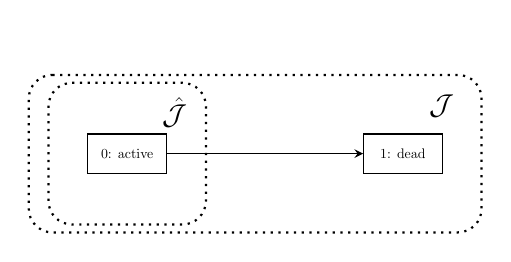
\begin{tikzpicture}[scale = 0.5, transform shape]
		\begin{scope}[every node/.style={ minimum width = 2cm, minimum height = 1cm}]
		\node (0) [rectangle, draw] at (0, 0) {$\text{0: active}$};
		\node (1) [rectangle, draw] at (7, 0) {$\text{1: dead}$};

		\end{scope}
		
		\begin{scope}[every node/.style={minimum width = 2cm, minimum height = 4cm}]
		\node (34) at (8, 1.2) {\fontsize{20}{30}\selectfont $\mathcal{J}$};
		\end{scope}
		
		\begin{scope}[every node/.style={minimum width = 2cm, minimum height = 4cm}]
		\node (33) at (1.2, 1.05) {\fontsize{20}{30}\selectfont $\hat{\mathcal{J}}$};
		\end{scope}
		
		\begin{scope}[>={stealth[black]},
		every edge/.style = {draw = black}]
		\path [->] 	(0) edge [] node {} (1);
		\end{scope}
		
		

		
		\draw [rounded corners = 3mm, thick, dotted, scale=1]
		($(0) + (-2.5, 2)$) --
		($(0) + (9, 2)$) --
		($(0) + (9, -2)$) --
		($(0) + (-2.5, -2)$)
		--cycle;
		
		\draw [rounded corners = 3mm, thick, dotted, scale=1]
		($(0) + (-2, 1.8)$) --
		($(0) + (2, 1.8)$) --
		($(0) + (2, -1.8)$) --
		($(0) + (-2, -1.8)$)
		--cycle;
		
		\end{tikzpicture}
		\caption{Alive-dead model}
	\end{center}
\end{figure}

For the time $t$ sojourn benefit rate prognosis, we condition on the policy holder not having died before time $t$ (because the events where she has already died by then doesn't interest her with respect to her prognoses). So we let $\hat{\mathcal{J}} = \{ 0 \}$ and the prognosis is

\begin{align*}
    \econd[b_{Z(t-)}(t)]{Z(t-) \in \hat{\mathcal{J}}} = \econd[b_0(t)]{Z(t-) = 0},
\end{align*}

which is the same conditioning as the classical prognoses. Likewise for the retirement lump sum prognosis:

\begin{align*}
    \econd[\triangle b_{Z(R-)}(R)]{Z(R-) \in \hat{\mathcal{J}}} = \econd[\triangle b_0(R)]{Z(R-) = 0},
\end{align*}

which is also the classical conditioning. With regard to the only transition benefit prognosis, the state $1$ transition, we have

\begin{align*}
\econd[b_{Z(t-)1}(t)]{Z(t-) \in \hat{\mathcal{J}}, Z(t)=1} =& \econd[b_{01}(t)]{Z(t-)=0, Z(t)=1} \\
=& \econd[b_{01}(t)]{\triangle N_1(t) = 1},
\end{align*}

This prognosis gives the policy holder an estimate of what she will leave to her bereaved in the event of her death \textit{exactly} at time $t$.

Example \ref{ExampleOne} demonstrates that in the alive-death model, the conditioning approach proposed doesn't really bring anything new to the table, as it coincides with the classical conditioning of staying active until payout time $t$. This is because "not dying" is the same event as "staying active". This is no longer the case in the active-disabled-death model, as the next example shows.

\subsubsection{The Disability Model} \label{DisModel}

Consider the active-disabled-dead model:

\begin{figure}[H]
	\begin{center}
		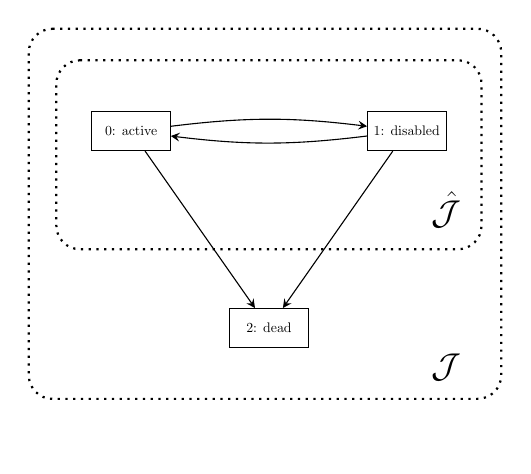
\begin{tikzpicture}[scale = 0.5, transform shape]
		\begin{scope}[every node/.style={ minimum width = 2cm, minimum height = 1cm}]
		\node (0) [rectangle, draw] at (0, 0) {$\text{0: active}$};
		\node (1) [rectangle, draw] at (7, 0) {$\text{1: disabled}$};
		\node (2) [rectangle, draw] at (3.5, -5) {$\text{2: dead}$};
;

		\end{scope}
		
		\begin{scope}[every node/.style={minimum width = 2cm, minimum height = 4cm}]
		\node (5) at (8, -2) {\fontsize{50}{60}\selectfont $\hat{\mathcal{J}}$};
		\end{scope}
		
		\begin{scope}[every node/.style={minimum width = 2cm, minimum height = 4cm}]
		\node (5f) at (8, -6) {\fontsize{50}{60}\selectfont $\mathcal{J}$};
		\end{scope}
		
		\begin{scope}[>={stealth[black]},
		every edge/.style = {draw = black}]
		\path [->] 	(0) edge [bend left = 7] node {} (1)
		(0) edge [] node {} (2)
		(1) edge [] node {} (2)
			(1) edge [bend left = 7] node {} (0);
		\end{scope}
		
		

		
		\draw [rounded corners = 3mm, thick, dotted, scale=1]
		($(2) + (-5.4, 6.8)$) --
		($(2) + (5.4, 6.8)$) --
		($(2) + (5.4, 2)$) --
		($(2) + (-5.4, 2)$)
		--cycle;
		
		\draw [rounded corners = 3mm, thick, dotted, scale=1]
		($(2) + (-6.1, 7.6)$) --
		($(2) + (5.9, 7.6)$) --
		($(2) + (5.9, -1.8)$) --
		($(2) + (-6.1, -1.8)$)
		--cycle;
		
		\end{tikzpicture}
		\caption{Active-disabled-dead model.}
		\label{fig: 3state}
	\end{center}
\end{figure}

In this model, most classical prognoses -- e.g. \cite{NinnaReitzel} -- condition on the policy holder staying active all the way up to the time of payout $t$, e.g. the event $\left( Z(s) 0 : 0 \leq s < t \right)$. Instead we only assume that the policy holder does not die -- she might become disabled. So we let $\hat{\mathcal{J}} = \{ 0, 1 \}$, such that the time $t$ sojourn benefit prognosis becomes

\begin{align*}
    \econd[b_{Z(t-)}(t)]{Z(t-) \in \hat{\mathcal{J}}}.
\end{align*}

Again, and for the same reason as given above, this conditioning excludes death before time $t$. However, it retains two important elements of risk that the classical conditioning does not:

\begin{itemize}
    \item The time $t$ sojourn benefit rate may not be the same in states 0 and 1, e.g. $b_0 \neq b_1$.
    \item The benefit may also depend on the past state path $\{ Z(s) \}_{0 \leq s < t}$, which is fixed in the classical conditioning, but only restricted to $\hat{\mathcal{J}}$ in the proposed conditioning. This means that $Z$ may leave the premium paying state 0 for periods before $t$, which for some types of contracts may reduce the benefit at time $t$.
\end{itemize}

The same arguments go for the retirement lump sum benefit prognosis, which is simply

\begin{align*}
\econd[\triangle B_{Z(R-)}(R)]{Z(R-) \in \hat{\mathcal{J}}}.
\end{align*}

With respect to the transition prognosis for the dead state $2$, the policy holder is interested in knowing what she can expect to have paid out to her bereaved in case of her death at time $t$. The prognosis is

\begin{align} \label{FirstTransProg}
    \econd[b_{Z(t-)2}(t)]{Z(t-) \in \hat{\mathcal{J}}, Z(t)=2},
\end{align}

which is the expected death sum paid out given death at exactly time $t$. The prognosis takes into account that the transition can be made from state 0 or from state 1 (which matters if $b_{02} \neq b_{12}$), and that the state process can have moved freely between 0 and 1 up until $t$, which for some contracts affect the benefit paid out.

The advantages of the proposed conditioning showed themselves already in the active-disabled-death model just presented. However, as we move to a more complex model with policy holder options, new interesting choices for $\hat{\mathcal{J}}$ show up.

\subsubsection{Multi-State Model With Policy Holder Options}

Consider a multi-state model with policy holder options:

	\begin{figure}[H]
		\begin{center}
			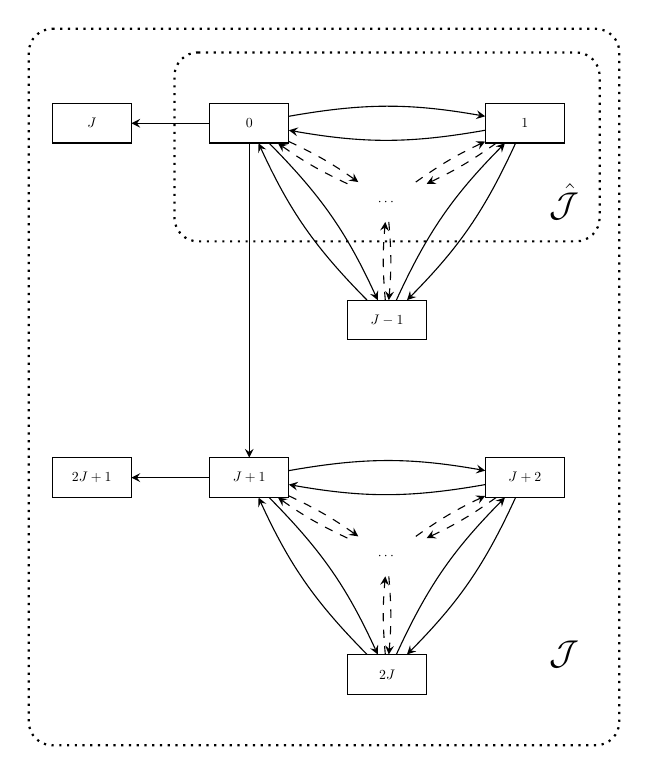
\begin{tikzpicture}[scale = 0.5, transform shape]
			\begin{scope}[every node/.style={ minimum width = 2cm, minimum height = 1cm}]
			\node (0) [rectangle, draw] at (0, 0) {0};
			\node (1) [rectangle, draw] at (7, 0) {1};
			\node (2) [rectangle, draw] at (3.5, -5) {$J - 1$};
			\node (3) [rectangle, dashed] at (3.5, -2) {$\cdots$};
			\node (4) [rectangle, draw] at (-4, 0) {$J$};
			\end{scope}
			
			\begin{scope}[every node/.style={minimum width = 2cm, minimum height = 4cm}]
			\node (5) at (8, -2) {\fontsize{50}{60}\selectfont $\hat{\mathcal{J}}$};
			\end{scope}
			
			\begin{scope}[every node/.style={minimum width = 2cm, minimum height = 1cm}]
			\node (0f) [rectangle, draw] at (0,-9) {$J + 1$};
			\node (1f) [rectangle, draw] at (7, -9) {$J + 2$};
			\node (2f) [rectangle, draw] at (3.5,-14) {$2J$};
			\node (3f) [rectangle, dashed] at (3.5, -11) {$\cdots$};
			\node (4f) [rectangle, draw] at (-4, -9) {$2J + 1$};
			\end{scope}
			
			\begin{scope}[every node/.style={minimum width = 2cm, minimum height = 4cm}]
			\node (5f) at (8, -13.5) {\fontsize{50}{60}\selectfont $\mathcal{J}$};
			\end{scope}
			
			\begin{scope}[>={stealth[black]},
			every edge/.style = {draw = black}]
			\path [->] 	(0) edge [bend left = 10] node {} (1)
			(1) edge [bend left = 10] node {} (0)
			(0) edge [bend left = 10] node {} (2)
			(2) edge [bend left = 10] node {} (0)
			(1) edge [bend left = 10] node {} (2)
			(2) edge [bend left = 10] node {} (1)
			(0) edge node {} (4);
			\end{scope}
			
			
			\begin{scope}[>={stealth[black]},
			every edge/.style = {draw = black, dashed}]
			\path [->] 	(0) edge [bend left = 5] node {} (3)
			(3) edge [bend left = 5] node {} (0)
			(1) edge [bend left = 5] node {} (3)
			(3) edge [bend left = 5] node {} (1)
			(2) edge [bend left = 5] node {} (3)
			(3) edge [bend left = 5] node {} (2);
			\end{scope}
			
			\begin{scope}[>={stealth[black]},
			every edge/.style = {draw = black}]
			\path [->] 	(0) edge node {} (0f);
			\end{scope}
			
			\begin{scope}[>={stealth[black]},
			every edge/.style = {draw = black}]
			\path [->] 	(0f) edge [bend left = 10] node {} (1f)
			(1f) edge [bend left = 10] node {} (0f)
			(0f) edge [bend left = 10] node {} (2f)
			(2f) edge [bend left = 10] node {} (0f)
			(1f) edge [bend left = 10] node {} (2f)
			(2f) edge [bend left = 10] node {} (1f)
			(0f) edge node {} (4f);
			\end{scope}
			
			\begin{scope}[>={stealth[black]},
			every edge/.style = {draw = black, dashed}]
			\path [->] 	(0f) edge [bend left = 5] node {} (3f)
			(3f) edge [bend left = 5] node {} (0f)
			(1f) edge [bend left = 5] node {} (3f)
			(3f) edge [bend left = 5] node {} (1f)
			(2f) edge [bend left = 5] node {} (3f)
			(3f) edge [bend left = 5] node {} (2f);
			\end{scope}
			
			\draw [rounded corners = 3mm, thick, dotted, scale=1]
			($(2) + (-5.4, 6.8)$) --
			($(2) + (5.4, 6.8)$) --
			($(2) + (5.4, 2)$) --
			($(2) + (-5.4, 2)$)
			--cycle;
			
			\draw [rounded corners = 3mm, thick, dotted, scale=1]
			($(2f) + (-9.1, 16.4)$) --
			($(2f) + (5.9, 16.4)$) --
			($(2f) + (5.9, -1.8)$) --
			($(2f) + (-9.1, -1.8)$)
			--cycle;
			
			\end{tikzpicture}
			\caption{Multi-state model with policy holder options}
			\label{fig: multi_state_model}
		\end{center}
	\end{figure}

In this model, we let $\hat{\mathcal{J}} = \{ 0, 1, ..., J-2 \}$. In words, we condition on the policy holder not having died, surrendered or converted to free policy until time $t$. The difference to the classical prognoses is -- again -- that the policy holder is no longer assumed to be active from the time of prognostication to the time of payment. Indeed, she may lose her ability to work -- or she may simply lose her job for a period (if the state space includes a "not employed" state). Both are relevant events to take into consideration when presenting her a prognosis.

The reason for excluding the surrender and free policy states from $\hat{\mathcal{J}}$ is not the same as the reason for excluding death. The policy holder is in control of the surrender and free policy transitions. So to her the transitions are not risks at all and shouldn't be treated as such when communicating prognoses. In contrast -- from the point of view of a company doing valuation or solvency calculations -- the transitions are risks and should be treated as such.

The relevant sojourn benefit prognosis and retirement lump sum prognosis are, respectively, 

\begin{align*}
&\econd[b_{Z(t-)}(t)]{Z(t-) \in \hat{\mathcal{J}}} \\
&\econd[\triangle B_{Z(R-)}(R)]{Z(R-) \in \hat{\mathcal{J}}},
\end{align*}

i.e. the expected rate (respectively lump sum) paid out at time $t$ (respectively time $R$), given that the policy holder has not died, surrendered or invoked the free policy option until time $t$.

An interesting prognosis for the surrender payment is

\begin{align*}
\econd[b_{0J}(t)]{Z(t-) \in \hat{\mathcal{J}}, Z(t)=J}.
\end{align*}

for $t \in [0,n]$ the time of surrender. This is exactly the expected sum paid out upon surrender at time $t$, given that the policy holder has not died, surrendered or invoked the free policy option up until time $t$.

Likewise, a prognosis for the free policy factor $\rho$ is

\begin{align*}
\econd[\rho(t)]{(Z(s) \in \hat{\mathcal{J}}, s<t) \cup (Z(t)=J+1)}.
\end{align*}

for $t \in [t_0,n]$ the time of free policy conversion. We stress again that these prognoses are only really interesting, if the surrender payment $b_{0J}(t)$ and the free policy factor $\rho(t)$ depend on the past state path $\{ Z(s) \}_{0 \leq s \leq t}$, which is not always the case.

\begin{remark}
	Remark on Markov and conditioning until time $n$.
\end{remark}


\begin{remark}
Remark on transitions inside $\hat{\mathcal{J}}$. Trick med at $\sigma(Z(t))=F^Z(t)$ for nogle kæder
\end{remark}

In the preceding chapter, we have motivated and presented definitions for three different prognoses, one for each type of payment typical for life insurance contracts:

\begin{itemize}
	\item Sojourn benefit rate prognoses (def. XX).
	\item Retirement lump sum benefit prognoses (def. XX).
	\item Transition benefit prognoses (def. XX).
\end{itemize}

In the two following chapters, the focus is on the computation of these prognoses. Chapter \ref{ChapGuaranteedBen} deals with the prognostication of guaranteed payments. In this case, closed form expressions

In Chapter \ref{ChapReserveDepBen}, we deal with the case of reserve-dependent benefits, which encompasses many popular contract types, including Unit Link and Participating Life Insurance. In this case, 

\newpage
\section{Prognoses -- Nominal benefits} \label{ChapGuaranteedBen}

In this chapter, we calculate the prognoses presented in Chapter 3 for a life insurance contract with nominal payments only. By \textit{nominal}, we mean that all payments are settled at the signing of the contract in accordance with the equivalence principle. Thus the payments at time $T$ do not depend on the the past state path of the policy holder $\{ Z(s) \}_{0 < s < T}$ or on any financial performance, but only on the state at payment time,  i.e. $Z(T-)$. As we shall see, this feature gives the prognoses a particularly simple form compared to the case of reserve-dependent benefits.

The chapter is structured as follows:

\begin{itemize}
	\item First, we calculate the three fixed path prognoses. The results are trivial.
	\item Second, we compute the three restricted path prognoses. The results are easily obtained and have intuitive interpretations.
	\item Finally, we close the chapter with a numerical example demonstrating the difference between the fixed- and the restricted path approaches.
\end{itemize}

\subsection{Fixed Path}

In the case of nominal benefits, the rates depend solely on the state of the policy holder at payment time $t$ or $R$ (and $t-$ for transition benefits). This information is obviously known in the fixed path conditioning and so the prognoses are trivially

\begin{align*}
	\econd[b_{Z(t)}(t)]{Z(s) = z(s) : 0 \leq s \leq t} =& b_{z(t)}(t), \\
	\econd[\triangle B_{Z(R)}(R)]{Z(s) = z(s) : 0 \leq s \leq R} =& \triangle B_{z(R)}(R), \\
	\econd[b_{Z(t-)k}(t)]{ Z(s) = z(s) : 0 \leq s \leq t} =& \1{z(t-) \neq k} \1{z(t) = k} b_{z(t-) k}(t),
\end{align*}

for some $k \in \mathcal{J}$ and some deterministic function $z: [0,t] \to \mathcal{J}$.

\subsection{Restricted Path}

In the case of restricted path conditioning, it it not known in which state the policy holder is at time of payout -- only that she is in the subset $\hat{\mathcal{J}} \subset \mathcal{J}$. The prognoses are then readily calculated:

\begin{proposition} \label{SojournWithoutBonus}
The time $t$ sojourn benefit rate prognosis in the case with guaranteed benefits is given by

\begin{align*}
    \econd[b_{Z(t-)}(t)]{Z(t-) \in \hat{\mathcal{J}}}
    &= \frac{\sum_{j \in \hat{\mathcal{J}}} p_{0j}(0,t) b_j(t)}{\sum_{j \in \hat{\mathcal{J}}} p_{0j}(0,t)}
\end{align*}
for some subset $\hat{\mathcal{J}} \subset \mathcal{J}$.
\end{proposition}

\begin{proof}
\begin{align*}
   	\econd[b_{Z(t-)}(t)]{Z(t-) \in \hat{\mathcal{J}}} &= \sum_{j \in \mathcal{J}} \econd[\1{Z(t-)=j}]{Z(t-) \in \hat{\mathcal{J}}} b_j(t) \\
    &= \frac{\sum_{j \in \hat{\mathcal{J}}} \expec[ 1_{\{Z(t-)=j\}} ] b_j(t)}{\probability[Z(t-) \in \hat{\mathcal{J}}]} \\
    &= \frac{\sum_{j \in \hat{\mathcal{J}}} p_{0j}(0,t) b_j(t)}{\sum_{j \in \hat{\mathcal{J}}} p_{0j}(0,t)}
\end{align*}

where we used the continuity of $p_{0j}(0,t)$.
\end{proof}

We see that the prognosis is simply the weighted average over $j \in \hat{\mathcal{J}}$ of the sojourn payment functions $b_j(t)$, with weights given by the probability of being in state $j$ at time $t$ (recall that $\hat{\mathcal{J}}$ is to be thought of as the full state space less the surrender, free policy and death state). The reason for this simplicity is that the only risk the policy holder is exposed to, is her state at time $t$. Since all the payments are fixed in the contract, it makes no difference e.g. how long she has been in a premium paying state, or how many times she has become disabled.

The retirement lump sum prognosis takes a similar form:

\begin{proposition} \label{RetireWithoutBonus}
The retirement lump sum prognosis in the case without bonus is given by

\begin{align*}
    \expec[ \triangle b_{Z(R-)}(R) | Z(R-) \in \hat{\mathcal{J}}]
    &= \frac{\sum_{j \in \hat{\mathcal{J}}} p_{0j}(0,R) \triangle b_j(R)}{\sum_{j \in \hat{\mathcal{J}}} p_{0j}(0,R)},
\end{align*}

for some subset $\bar{\mathcal{J}} \subset \mathcal{J}$.
\end{proposition}

\begin{proof}
\begin{align*}
	\econd[\triangle b_{Z(R-)}(R)]{Z(R-) \in \hat{\mathcal{J}}} &= \sum_{j \in \mathcal{J}} \econd[\1{Z(R-)=j}]{Z(R-) \in \hat{\mathcal{J}}} \triangle b_j(R) \\
	&= \frac{\sum_{j \in \hat{\mathcal{J}}} \expec[ 1_{\{Z(R-)=j\}} ] \triangle b_j(R)}{\probability[Z(R-) \in \hat{\mathcal{J}}]} \\
	&= \frac{\sum_{j \in \hat{\mathcal{J}}} p_{0j}(0,R) \triangle b_j(R)}{\sum_{j \in \hat{\mathcal{J}}} p_{0j}(0,R)}
\end{align*}

where we again used the continuity of $p_{0j}(0,t)$.
\end{proof}

Again, the prognosis is simply a weighted average of the lump sum payouts of the states $j$, with weights given by the probability of being in state $j$ at time of retirement $R$.

\begin{remark}[Reducing the state space] \label{ReducedStateSpace}
We can arrive at these two first prognoses -- sojourn and retirement lump sum -- via a slightly different approach. Define a new Markov chain $\hat{Z}$ on the state space $\hat{\mathcal{J}}$ with transition probabilities SLET MÅSKE

\begin{align*}
    \hat{p}_{ij}(s,t) =& \pcond[\hat{Z}(t) = j]{\hat{Z}(s) = i} \\
    :=& \frac{p_{ij}(s,t)}{\sum_{j \in \hat{\mathcal{J}}} p_{ij}(s,t)}, \, \, \, \, \, i,j \in \hat{\mathcal{J}}, \, \, s < t,
\end{align*}

We then obtain the sojourn prognosis

\begin{align*}
    \expec[b_{\hat{Z}(t)}(t)] =& \sum_{j \in \hat{\mathcal{J}}} \hat{p}_{0j}(0,t) b_j(t) \\
    =& \frac{\sum_{j \in \hat{\mathcal{J}}} p_{0j}(t_0,t) b_j(t)}{\sum_{j \in \hat{\mathcal{J}}} p_{0j}(t_0,t)},
\end{align*}

which is identical to Proposition \ref{SojournWithoutBonus}. So the sojourn and retirement lump sum prognoses can be obtained by reducing the state space and normalizing the transition probabilities accordingly. However, as we shall see, this approach does not work for the transition prognoses, because the intensities out of $\hat{\mathcal{J}}$ matter. So reducing the chain from $Z$ to $\hat{Z}$ throws away needed information.
\end{remark}

As we have seen, the transition benefit prognosis takes a slightly different form, as the conditioning event differs from the sojourn and the lump sum case -- recall the discussion in Section \ref{CondForProg}. To calculate the transition prognoses, we need a lemma:

\begin{lemma} \label{Split}
	Given an $F^Z$-adapted process W, we have for $j \in \hat{\mathcal{J}}$ and $k \notin \hat{\mathcal{J}}$
	
	\begin{align*}
		\econd[\1{Z(t-)=j} W(t-)]{Z(t-) \in \hat{\mathcal{J}}, Z(t) = k} =& \frac{\sum_{j \in \hat{\mathcal{J}}} \expec[\1{Z(t-)=j} W(t-)] \mu_{jk}(t)}{\sum_{j \in \hat{\mathcal{J}}} p_{0j}(t_0,t) \mu_{jk}(t)}
	\end{align*}
\end{lemma}
\begin{proof}
	See Appendix \ref{SplitProof}.
\end{proof}

The prognosis now follows:

\begin{proposition} \label{TransitionWithoutBonus}
The state $k$ transition benefit prognosis in the case without bonus is given by

\begin{align*}
    \econd[b_{Z(t-)k}(t)]{Z(t-) \in \hat{\mathcal{J}}, Z(t)=k} = \frac{\sum_{j \in \hat{\mathcal{J}}} p_{0j}(0,t) \mu_{jk}(t) b_{jk}(t)}{\sum_{j \in \hat{\mathcal{J}}} p_{0j}(0,t) \mu_{jk}(t)},
\end{align*}

for some subset $\bar{\mathcal{J}} \subset \mathcal{J}$ and $k \notin \bar{\mathcal{J}}$.
\end{proposition}
\begin{proof}
The result follows immediately from Lemma \ref{Split} (letting $W=0$) since

\begin{align*}
	\econd[b_{Z(t-)k}(t)]{Z(t-) \in \hat{\mathcal{J}}, Z(t)=k} =& \sum_{j \in \hat{\mathcal{J}}} \econd[\1{Z(t-)=j}]{Z(t-) \in \hat{\mathcal{J}}, Z(t) = k} b_{jk}(t) \\
	=&\frac{\sum_{j \in \hat{\mathcal{J}}} \expec[\1{Z(t-)=j}] \mu_{jk}(t) b_{jk}(t)}{\sum_{j \in \hat{\mathcal{J}}} p_{0j}(0,t) \mu_{jk}(t)} \\
	=&\frac{\sum_{j \in \hat{\mathcal{J}}} p_{0j}(0,t) \mu_{jk}(t) b_{jk}(t)}{\sum_{j \in \hat{\mathcal{J}}} p_{0j}(0,t) \mu_{jk}(t)},
\end{align*}

where we also used the continuity of $p_{0j}(0,t)$
\end{proof}

Again, the prognosis take the form of a weighted average of payment functions $b_{jk}(t)$. This time, however, the weights are the probabilities -- given a transition into state $k$ at time $t$ -- that the transition happened from state $j$. These weights $p_{0j}(0,t) \mu_{jk}(t)$ resemble probability density functions -- i.e. the (generalized) survival function $p_{0j}(0,t)$ times the intensity $\mu_{jk}(t)$. This is rather intuitive, since what we're after is the probability of making the transition $j \mapsto k$ in a small time interval around $t$.

\begin{remark}
	From Propositions XX, XX and XX, it is clear that the problem of calculating prognoses in the case without bonus is only as complex as calculating the transition probabilities $p_{0j}(0,t)$. Outside of very simple models, where these probabilities can be found analytically, this requires solving the Kolmogorov forward differential equations in a one-dimensional time grid. As we shall see the case with bonus requires solving a forward differential equation containing the transition probabilities....
\end{remark}

\subsection{Examples}

We close this chapter by giving two examples of contracts with nominal benefits, where the fixed path prognoses differ from the restricted path prognoses. The examples are simple, but are meant to inspire confidence that the idea of restricted path conditioning is a sound one before moving on to more complex contracts in the next chapter.

Both examples are modelled on the classical active-disabled-dead model with reactivation:

\begin{figure}[H]
	\begin{center}
		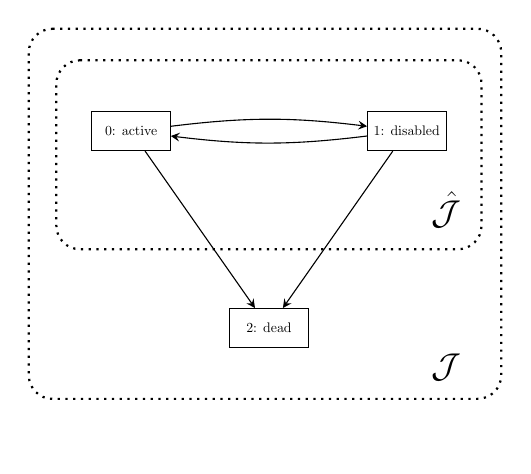
\begin{tikzpicture}[scale = 0.5, transform shape]
		\begin{scope}[every node/.style={ minimum width = 2cm, minimum height = 1cm}]
		\node (0) [rectangle, draw] at (0, 0) {$\text{0: active}$};
		\node (1) [rectangle, draw] at (7, 0) {$\text{1: disabled}$};
		\node (2) [rectangle, draw] at (3.5, -5) {$\text{2: dead}$};
		;
		
		\end{scope}
		
		\begin{scope}[every node/.style={minimum width = 2cm, minimum height = 4cm}]
		\node (5) at (8, -2) {\fontsize{50}{60}\selectfont $\hat{\mathcal{J}}$};
		\end{scope}
		
		\begin{scope}[every node/.style={minimum width = 2cm, minimum height = 4cm}]
		\node (5f) at (8, -6) {\fontsize{50}{60}\selectfont $\mathcal{J}$};
		\end{scope}
		
		\begin{scope}[>={stealth[black]},
		every edge/.style = {draw = black}]
		\path [->] 	(0) edge [bend left = 7] node {} (1)
		(0) edge [] node {} (2)
		(1) edge [] node {} (2)
		(1) edge [bend left = 7] node {} (0);
		\end{scope}
		
		
		
		
		\draw [rounded corners = 3mm, thick, dotted, scale=1]
		($(2) + (-5.4, 6.8)$) --
		($(2) + (5.4, 6.8)$) --
		($(2) + (5.4, 2)$) --
		($(2) + (-5.4, 2)$)
		--cycle;
		
		\draw [rounded corners = 3mm, thick, dotted, scale=1]
		($(2) + (-6.1, 7.6)$) --
		($(2) + (5.9, 7.6)$) --
		($(2) + (5.9, -1.8)$) --
		($(2) + (-6.1, -1.8)$)
		--cycle;
		
		\end{tikzpicture}
		\caption{Active-disabled-dead model}
		\label{fig: 3state}
	\end{center}
\end{figure}

\subsubsection{A Retirement Lump Sum Contract}

Assume a contract paying out the lump sum $\triangle B_0$ if the policy holder is active at the time of retirement $R$. If the she is disable at retirement, she receive no benefit. Premium $\pi$ is paid as active until retirement. In other words, the payment stream is

\begin{align*}
	dB(t) =& \1{t<R} \1{Z(t)=0)} \pi dt + \1{Z(t)=0} \triangle B_0 d \varepsilon_R(t),
\end{align*}

with payments balanced under technical fairness, i.e. $V_0^*(0)=0$.

Choosing for the fixed path prognosis the path $z(s) = 0$, $s \leq R$ i.e. that the policy holder remains active until retirement, we obviously have

\begin{align} \label{Fixed}
	\econd[\triangle B_{Z(R)}(R)]{Z(s) = z(s) : 0 \leq s \leq R} =& \triangle B_0,
\end{align}

Compare this to the restricted path prognosis with restricting subset $\hat{\mathcal{J}} = \{ 0,1 \}$, i.e. that the policy holder survives until retirement. By Proposition \ref{RetireWithoutBonus},

\begin{align} \label{Restricted}
\begin{split}
		\econd[\triangle B_{Z(R)} (R)]{Z(R) \in \{ 0,1 \}} =& \frac{\sum_{j = 0}^1 p_{0j}(0,R) \triangle B_j(R)}{\sum_{j = 0}^1 p_{0j}(0,R)} \\
	=&\frac{p_{00}(0,R) \triangle B_0 + p_{01}(0,R) \cdot 0}{p_{00}(0,R) + p_{01}(0,R)} \\
	=& \frac{p_{00}(0,R)}{p_{00}(0,R) + p_{01}(0,R)} \triangle B_0 \\
	=& \pcond[Z(R) = 0]{Z(R) \in \{ 0,1 \}} \cdot \triangle B_0,
\end{split}
\end{align}

which is just the probability of staying active until retirement (given survival until retirement) times the lump sum $\triangle B_0$ rewarded for doing so. Obviously, the restricted path prognosis in (\ref{Restricted}) is more conservative than the fixed path prognosis in (\ref{Fixed}).

Defining the transition intensities (taken from Section 5 of \cite{BuchardtMoller})

\begin{align} \label{Intensities}
\begin{split}
		\mu_{01}(t) =& \left(0.0004 + 10^{4.54 + 0.06t - 10}\right) \1{t<R}, \\
	\mu_{10}(t) =& \left(2.0058 \cdot e^{-0.117t}\right) \1{t<R}, \\
	\mu_{02}(t) =& 0.0005 + 10^{5.88 + 0.038t - 10}, \\
	\mu_{12}(t) =& \mu_{02}(t) \left( 1 + \1{t<R} \right),
\end{split}
\end{align}

and setting $\triangle B_0=1$, we illustrate the two prognoses in the following figure:

\begin{figure}[H]
	\centering
	\caption{Lump sum prognoses (fixed- and restricted path conditioning)}
	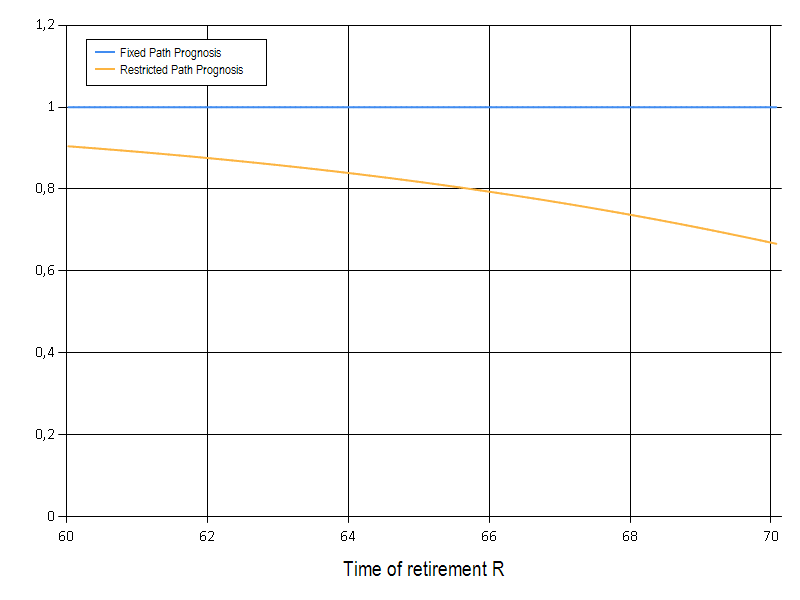
\includegraphics[width=\textwidth]{LumpSum} \label{LumpFigure}
\end{figure}

Figure \ref{LumpFigure} shows that not only is the restricted path prognosis the more conservative of the two -- the difference is also larger for higher retirement ages. This is because the disability intensity $\mu_{01}$ in this example is increasing and the reactivation intensity $\mu_{10}$ decreasing. Consequently, the probability of being active at retirement -- given survival until retirement -- is decreasing.

The example shows that for certain contracts the fixed path prognosis can overestimate the benefit paid out.

\subsubsection{A Term Insurance Contract}

Next, consider a contract paying out the sum insured $b_{02}$ if the policy holder is active at the time of death. If she she dies as disabled, no benefit is paid out. Premium $\pi$ is paid as active until retirement. The payment stream is

\begin{align*}
	dB(t) =& \1{t<R} \1{Z(t)=0)} \pi dt + \1{t<R} \1{Z(t-)=0} b_{02} d N_2(t),
\end{align*}

with payments determined under technical fairness, i.e. $V_0^*(0)=0$.

Letting $0<T<R$ denote the time of death, we choose for the fixed path prognosis the path $z(s) = \1{s \geq T} \cdot 2$, i.e. that the policy remains active until the time of death. The prognosis is trivially

\begin{align} \label{Fixed2}
	\econd[b_{Z(T-)2}(T)]{ Z(s) = z(s) : 0 \leq s \leq T} =& b_{02}
\end{align}

In contrast, the restricted path prognosis with restricting subset $\hat{\mathcal{J}} = \{ 0,1 \}$ -- i.e. that the policy holder may become disabled before dying -- is by Proposition \ref{TransitionWithoutBonus},

\begin{align} \label{Restricted2}
\begin{split}
	\econd[b_{Z(t-)2}(t)]{Z(t-) \in \{ 0,1 \}, Z(t)=2} =& \frac{\sum_{j=0}^1 p_{0j}(0,t) \mu_{j2}(t) b_{j2}(t)}{\sum_{j=0}^1 p_{0j}(0,t) \mu_{j2}(t)} \\
	=&\frac{p_{00}(0,t) \mu_{02}(t) b_{02} + p_{01}(0,t) \mu_{12}(t) \cdot 0}{p_{00}(0,t) \mu_{02}(t) + p_{01}(0,t) \mu_{12}(t)} \\
	=&\frac{p_{00}(0,t) \mu_{02}(t)}{p_{00}(0,t) \mu_{02}(t) + p_{01}(0,t) \mu_{12}(t)} b_{02},
\end{split}
\end{align}

which is again a weighted average of the transition payments with weights given by the 'densities' $p_{0j}(0,t) \mu_{j2}(t)$. As discussed earlier in the chapter, the intensities $\mu_{j2}(t)$ appear -- intuitively -- because given death at time $T$, it is more probable that the state from where death occurs is state $j$ if $\mu_{j2}(t)$ is large. Defining the transition intensities as (\ref{Intensities}) and setting $b_{02} = 1$, we illustrate the two prognoses in the following figure:

\begin{figure}[H]
	\centering
	\caption{Term insurance prognoses (fixed- and restricted path conditioning)}
	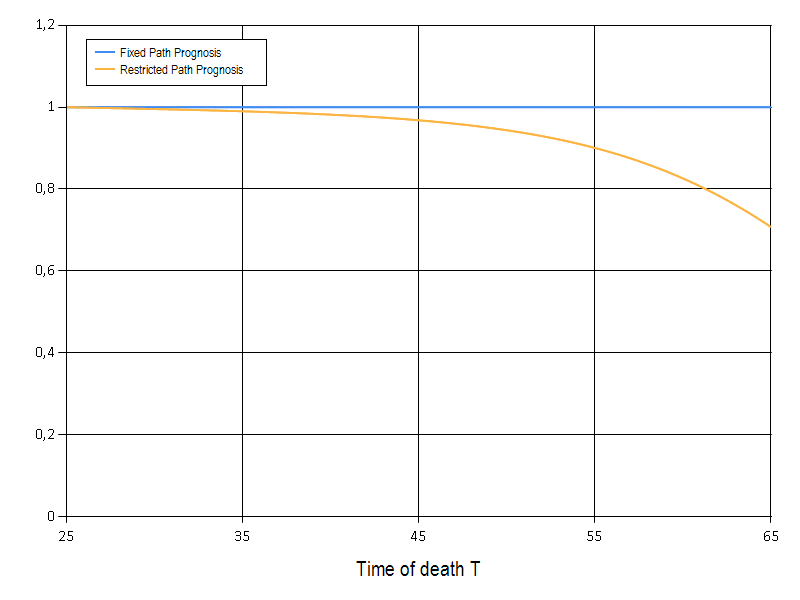
\includegraphics[width=\textwidth]{Term} \label{Term}
\end{figure}

As was the case for the lump sum prognosis, Figure \ref{Term} shows the restricted path prognosis to be the the more conservative of the two. For early time of death, the prognoses are nearly identical. This is partly because the probability of being disabled is very low, i.e. $p_{01}(0,T) \approx 0$ and partly because the mortalities are at about the same level, i.e. $\mu_{02}(T) \approx \mu_{12}(T)$ and so the quotient in (\ref{Restricted2}) is close to 1. As the time of death $T$ increases, so does $p_{01}(0,T)$ and the difference $\mu_{12}(T) - \mu_{02}(T)$, and so the quotient approaches 0.

The example shows, as did the former, that for certain contracts the fixed path prognosis can give a too optimistic picture of the future benefits.

In the preceding chapter, we saw how to calculate .

However, many modern insurance contracts include benefits that are not guaranteed, but instead depend on the performance of a number of individual or collective reserves and accounts. 

\subsubsection{Slet}

which is just the probability of staying active until retirement (given survival until retirement) times the lump sum $\triangle B_0$ rewarded for doing so. Obviously, the restricted path prognosis in (\ref{Restricted}) is more conservative than the fixed path prognosis in (\ref{Fixed}).

SLET MÅSKERecalling Remark \ref{ReducedStateSpace}, $\pcond[Z(R) = 0]{Z(R) \in \{ 0,1 \}}$ can be interpreted as the probability -- in a model with only two states: 0 and 1 -- of being in state 0 at time $t$. It is worth noting that this probability does not depend on the mortalities, $\mu_{02}$ and $\mu_{12}$.


The contract is specified as follows:

\begin{itemize}
    \item Before retirement, the policy holder pays a constant premium rate $\pi$ if active, and receives a constant disability benefit rate $b_1$ if disabled.
    \item In case of death before retirement, a transition lump sum is paid out to the bereaved: $b_{01}$ if she dies as active, $b_{12}$ if she dies as disabled.
    \item At retirement, she is paid a lump sum pension benefit $\triangle b_0$ if and only if she is active at the point of retirement $R$. As retired, she is paid a constant pension benefit $b_0=b_1$ as long as she remains alive.
\end{itemize}

Mathematically put, the payment stream takes the form

\begin{align*}
    dB(t) =& \1{t<R} \left( - \1{Z(t-)=0)} \pi + \1{Z(t-)=1} b_1 \right) dt \\
    &+ \1{t<R} \left( \1{Z(t-)=0} b_{02} + \1{Z(t-)=1} b_{12} \right) dN_2(t) \\
    &+ \1{Z(t-)=0} \triangle b_0 d \varepsilon_R(t) + \1{t \geq R} \1{Z(t-) \neq 2} b_0dt
\end{align*}

The payments are determined such that the equivalence principle is satisfied under the technical basis, i.e.

\begin{align*}
    \expecStar[\int_0^n e^{-\int_0^s r^*(u)du} dB(s)] = 0
\end{align*}

We can now calculate prognoses using Propositions \ref{SojournWithoutBonus}, \ref{RetireWithoutBonus} and \ref{TransitionWithoutBonus}. Due to the simplicity of the model and the payments, some prognoses are trivial. For instance, the sojourn pension benefit prognosis (so let $t \geq R$) is calculated with Proposition \ref{SojournWithoutBonus} as

\begin{align*}
    \econd[b_{Z(t-)} (t)]{Z(t-) \in \{ 0,1 \}} =& \frac{\sum_{j = 0}^1 p_{0j}(0,t) b_j(t)}{\sum_{j = 0}^1 p_{0j}(0,t)} \\
    =& b_0
\end{align*}

because the pension benefit $b$ is the same for the active and disabled states.

A nontrivial prognosis, however, is the retirement lump sum prognosis. By Proposition \ref{RetireWithoutBonus},

\begin{align*}
    \econd[\triangle b_{Z(R-)} (R)]{Z(R-) \in \{ 0,1 \}} =& \frac{\sum_{j = 0}^1 p_{0j}(0,R) \triangle b_j(R)}{\sum_{j = 0}^1 p_{0j}(0,R)} \\
    =&\frac{p_{00}(0,R) \triangle b_0 + p_{01}(0,R) \cdot 0}{p_{00}(0,R) + p_{01}(0,R)} \\
    =& \frac{p_{00}(0,R)}{p_{00}(0,R) + p_{01}(0,R)} \triangle b_0 \\
    =& \pcond[Z(R) = 0]{Z(R) \in \{ 0,1 \}} \cdot \triangle b_0,
\end{align*}
    
which is just the probability of staying active until retirement (given survival until retirement) times the lump sum $\triangle b_0$ rewarded for doing so. Recalling Remark \ref{ReducedStateSpace}, $\pcond[Z(R) = 0]{Z(R) \in \{ 0,1 \}}$ can be interpreted as the probability -- in a model with only two states: 0 and 1 -- of being in state 0 at time $t$. It is worth noting that this probability does not depend on the intensities out of $\hat{\mathcal{J}}$, $\mu_{02}$ and $\mu_{12}$.

If we assume that no reactivation can occur, i.e. $\mu_{10}=0$, the prognosis simplify to

\begin{align*}
\econd[\triangle b_{Z(R)} (R)]{Z(R) \in \{ 0,1 \}} =& \frac{p_{00}(0,R)}{p_{00}(0,R) + p_{01}(0,R)} \triangle b_0 \\
=& e^{-\int_0^t \mu_{01}(u)du} \triangle b_0,
\end{align*}

where the transition probabilities were found with Kolmogorovs forward differential equation\footnote{See Appendix \ref{KolmoProof} for proof.}. Again recalling Remark \ref{ReducedStateSpace}, this can be interpreted as the probability -- in a model with only two states: 0 and 1 -- of not making the transition from state $0$ to state $1$ before time $R$, times the lump sum reward for not doing so.

Finally, using Proposition \ref{TransitionWithoutBonus}, we can calculate the state $2$ transition prognosis, i.e. the expected death sum paid out given death at time $t<R$:

\begin{align*}
    \econd[b_{Z(t-)2}(t)]{Z(t-) \in \{ 0,1 \}, Z(t)=2} =& \frac{\sum_{j=0}^1 p_{0j}(0,t) \mu_{j2}(t) b_{j2}(t)}{\sum_{j=0}^1 p_{0j}(0,t) \mu_{j2}(t)} \\
    =&\frac{p_{00}(0,t) \mu_{02}(t) b_{02} + p_{01}(0,t) \mu_{12}(t) b_{12}}{p_{00}(0,t) \mu_{02}(t) + p_{01}(0,t) \mu_{12}(t)},
\end{align*}

which is again a weighted average of the transition payments with weights given by the 'densities' $p_{0j}(0,t) \mu_{j2}(t)$. In contrast to the retirement lump sum prognosis, the transition prognosis depends on the intensities out of $\hat{\mathcal{J}}$ -- i.e. $\mu_{02}$ and $\mu_{12}$ -- and so does not simplify nicely with the assumption of no reactivation.

However, if we also assume that $\mu_{02}=\mu_{12}$ the prognosis simplifies to

\begin{align*}
    \econd[b_{Z(t-)2}(t)]{Z(t-) \in \{ 0,1 \}, Z(t)=2} =&\frac{p_{00}(0,t) b_{02} + p_{01}(0,t) b_{12}}{p_{00}(0,t) + p_{01}(0,t)} \\
    =& e^{-\int_0^t \mu_{01}(u)du} b_{02} + \left(1 - e^{-\int_0^t \mu_{01}(u)du} \right) b_{12}
\end{align*}

which, again recalling Remark \ref{ReducedStateSpace}, can be interpreted as a weighted average in a two state model -- the first weight being the probability of there being no transition from state $0$ to state $1$ before $t$, the second being the probability of a transition taking place.

TABLE FOR COMPARISON

In the preceding chapter, we saw how to calculate .

However, many modern insurance contracts include benefits that are not guaranteed, but instead depend on the performance of a number of individual or collective reserves and accounts. 

\newpage
\section{Prognoses -- Reserve-Dependent Benefits} \label{ChapReserveDepBen}

In the preceding chapter, we saw how to calculate prognoses for nominal benefits, i.e. benefits that are completely determined at the signing of the contract and only depend on the state at the time of payment. This is overly restrictive, as many modern life and pension contracts include payments that are tied to the level of some reserves, accounts or other indices. We will here treat payment streams on the linear form

\begin{align} \label{TotalPaymentStream}
\begin{split}
	dB(t,W(t-)) =& W(t-) dB(t) \\
=& \sum_{i=1}^{m} W^i(t-) dB^i(t),
\end{split}
\end{align}

In other words, the $m$-dimensional vector $B$ consists of profile payment streams $B^i$ on the form (\ref{PaymentProcessDef}), which are then scaled linearly by the entries of the $\mathcal{F}$-adapted $m$-dimensional vector process $W$.

\begin{remark}
	Throughout the thesis, the product of two vectors of equal length shall always be understood in the sense (\ref{TotalPaymentStream}), i.e. as if the first vector is a row vector and the second a column vector.
\end{remark}

We will allow the process $W$ to have dynamics on the general form

\begin{align} \label{WDynamicsStart}
	\begin{split}
		dW(t) =& f_{Z(t-)}(t,W(t-)) dt \\
		&+ \sum_{k \in \mathcal{J} \atop k \neq Z(t-)} g_{Z(t-)k}(t,W(t-)) dN_{k}(t) \\
		&+ h_{Z(t-)}(t,W(t-)) d \varepsilon_R(t),
	\end{split}
\end{align}

for $n$-dimensional deterministic functions $f$, $g$ and $h$ of finite variation that are $\mathcal{C}^0$ on $(0,R) \cup (R,n)$ and on the form

\begin{align*}
	f_j(t,w) =& f_j^0(t) + f_j^1(t) \cdot w \\
	g_{jk}(t,w) =& g_{jk}^0(t) + g_{jk}^1(t) \cdot w \\
	h_j(t,w) =& h_j^0(t) + h_j^1(t) \cdot w,
\end{align*}

for $m \times m$-matrices $f_j^1$, $g_{jk}^1$ and $ h_j^1$ and vectors $f_j^0$, $g_{jk}^0$ and $ h_j^0$ of length $m$.

As we shall see, this affine dynamics structure is mathematically tractable enough that we can obtain the differential equations necessary to calculate prognoses \textit{and} general enough to encompass a large class of life insurance contracts.

The chapter is structured as follows:

\begin{itemize}
	\item We start out by formulating the theory in general terms and then show that the guaranteed benefits from the last chapter can be treated as a special case. 
	\item Then, we show that a broad class of With Profit contracts -- as presented in Chapter VI in \cite{Liv2Bog} -- also fits into the general theory, with $(X,Y)$ ($X$ being the technical reserve of guaranteed payments and $Y$ being the surplus) playing the role of $\textbf{W}$.
	\item Finally, the differences between the classical prognoses (without event risk) and the proposed are discussed in the context of a numerical example.
\end{itemize}



\subsection{Fixed Path}

The fixed path prognosis for reserve-dependent benefits -- with the path fixed in the active state -- is arguably the most common type of prognosis in the literature (e.g. \cite{NinnaReitzel}) and in the industry. It is the type pursued in \cite{Munk}, which forms the basis of the prognosis recommendation that the Danish pension and insurance industry association Forsikring \& Pension communicated to its members in 2018 (see \cite{Henstilling}). Consequently, it is the type of prognosis that most Danish life and pension companies offer their policy holders today.

The fixed path prognoses are straightforward to calculate. On the event

\begin{align*}
	\left( Z(s) = z(s) : 0 \leq s \leq n \right),
\end{align*}

for some deterministic function $z: [0,n] \to \mathcal{J}$, there is no event risk because $Z$ is completely determined. Then if the financial risk is handled scenario-wise (as in this thesis), there is no stochasticity left at all. So the dynamics in (\ref{WDynamicsStart}) can be recast as

\begin{align*}
	\begin{split}
		dW_z(t) =& f_{z(t-)}(t,W_z(t-)) dt \\
		&+ \sum_{k \in \mathcal{J} \atop k \neq z(t-)} g_{z(t-)k}(t,W_z(t-)) dn_{k}(t) \\
		&+ h_{z(t-)}(t,W_z(t-)) d \varepsilon_R(t),
	\end{split}
\end{align*}

where

\begin{align*}
	n_{k}(t) = \# \{ s \in (0,t] \, : \, z(s-) \neq k, z(s)=k \},
\end{align*}

is just the deterministic variant of $N_k(t)$. With $n_k(t)$ being deterministic, the transition payments happen at deterministic time points -- just the same as the retirement lump sum payment. Denote by $A(z) = \{ t \in (0,n] : z(t) \neq z(t-) \}$ the transition time points. Then $W_z$ is described by the differential equation

\begin{align} \label{Et}
	\frac{\partial}{\partial t} W_z(t) = f_{z(t-)}(t,W_z(t-))
\end{align}

for $t \in [0,n] \setminus \left( \{ R \} \cup A(z) \right)$. The initial value is $w_0$ and the gluing conditions are

\begin{align} \label{To}
\begin{split}
	W_z(R) =& W_z(R-) + h_{z(R-)}(R,W_z(R-)), \\
	W_z(u) =& W_z(u-) + g_{z(u-)z(u)}(u,W_z(u-)), \, \, \forall u \in A(z).
\end{split}
\end{align}

Having obtained the reserve $W_z$, the prognoses follow from equation (\ref{TotalPaymentStream}): Simply multiply $W_z$ with the respective payment functions $b_{z(t)}(t)$, $\triangle B_{z(R)}(R)$ and $b_{z(t-)k}(t)$. These considerations lead to the following proposition:

\begin{proposition} \label{FixedPath}
	Given a deterministic path $z: [0,n] \to \mathcal{J}$, the fixed path prognoses are given by
	
	\begin{align*}
		\hat{b}^{z}(t) =& W_z(t-)b_{z(t-)}(t) , \\
		\triangle \hat{B}^{z}(R) =& W_z(R-)\triangle B_{z(R-)}(R) , \\
		\hat{b}_{\cdot k}^{z}(t) =& \1{z(t-) \neq k} \1{z(t) = k} W_z(t-) b_{z(t-) k}(t) ,
	\end{align*}

where $W_z$ is a deterministic function described by equations (\ref{Et}) and (\ref{To}).
\end{proposition}

\begin{remark}
	A very common application of these fixed path prognoses is the simple Unit Link savings contract presented in \cite{Munk}. To replicate it in the current framework, simply let $m=1$, $z = 0$, $g=h=0$ and

\begin{align*}
	f_z(t-)(t,W_z(t-)) =
	\left\{
	\begin{array}{ll}
		\left( r(t) + \mu(t) \right) W_z(t) + \pi(t) & \mbox{if } t \in (0,R) \\
		\left( r(t) + \mu(t) - a^{-1}(t)) \right) W_z(t) & \mbox{if } t \in [R,n]
	\end{array}
	\right.
\end{align*}

where $\pi$ is premiums paid, $\mu$ is the mortality as active and $a$ is some payout annuity decided by the company. Having solved for $W_z$, the prognosis for the pension benefit is then simply

\begin{align*}
	\hat{b}^{z}(t) =& \frac{W_z(t-)}{a(t)}
\end{align*}

for $t \geq R$. This type of savings contract will be treated in greater detail in the example in Section \ref{Numerics}.
\end{remark}

\newpage
\subsection{Restricted Path}

The restricted path prognoses for reserve-dependent benefits are much more challenging prognoses to obtain than their fixed path counterparts. The difficulty stems from the fact that we no longer condition on the entire state path policy holder. We only assume that she remains in the subset $\hat{\mathcal{J}} \in \mathcal{J}$.

The restricted path prognoses for reserve-dependent benefits are given by

\begin{align*}
\hat{b}^{\hat{\mathcal{J}}}(T) =& \econd[W(t-) b_{Z(t-)}]{\{Z(s) \}_{0 \leq s < t} \in \hat{\mathcal{J}}} \\
\triangle \hat{B}^{\hat{\mathcal{J}}}(R) =& \econd[W(R-) \triangle B_{Z(R-)}]{\{Z(s) \}_{0 \leq s < R} \in \hat{\mathcal{J}}} \\
\hat{b}^{\hat{\mathcal{J}}}_{\cdot k}(t) =& \econd[W(t-) b_{Z(t-)k}]{\{Z(s) \}_{0 \leq s < t} \in \hat{\mathcal{J}}, Z(t) = k}
\end{align*}

Rewriting, we obtain for the sojourn benefit prognosis

\begin{align} \label{One}
	 \hat{b}^{\hat{\mathcal{J}}}(t) =& \econd[W(t-)b_{Z(t-)}]{\{Z(s) \}_{0 \leq s < t} \in \hat{\mathcal{J}}} \nonumber \\
	 =& \econd[W(t-)b_{Z(t-)}]{Z(t-) \in \hat{\mathcal{J}}} \nonumber \\
	 =&\frac{\sum_{j \in \hat{\mathcal{J}}} \expec[\1{Z(t-)=j} W(t-)] b_j(t)}{\probability[Z(t-) \in \hat{\mathcal{J}}]} \nonumber \\
	 =&\frac{\sum_{j \in \hat{\mathcal{J}}} \expec[\1{Z(t-)=j} W(t-)] b_j(t)}{\sum_{j \in \hat{\mathcal{J}}} p_{Z(t_0)j}(t_0,t)},
\end{align}

where we used Assumption (\ref{FirstAssump}). By the same arguments, the retirement lump sum prognosis is

\begin{align} \label{Two}
\triangle \hat{B}^{\hat{\mathcal{J}}}(R) =& \frac{\sum_{j \in \hat{\mathcal{J}}} \expec[\1{Z(R-)=j} W(R-)] \triangle B_j(R)}{\sum_{j \in \hat{\mathcal{J}}} p_{Z(t_0)j}(t_0,R)},
\end{align}

Finally, the state $k$ transition prognosis can be recast as

\begin{align} \label{Three}
\hat{b}_{\cdot k}^{\hat{\mathcal{J}}}(t) =& \econd[W(t-)b_{Z(t-)k}]{\{Z(s) \}_{0 \leq s < t} \in \hat{\mathcal{J}}, Z(t)=k} \nonumber \\
=& \econd[W(t-)b_{Z(t-)k}]{Z(t-) \in \hat{\mathcal{J}}, Z(t)=k} \nonumber \\
=& \sum_{j \in \hat{\mathcal{J}}} \econd[\1{Z(t-)=j} W(t-)]{Z(t-) \in \hat{\mathcal{J}}, Z(t) = k} b_{jk}(t) \nonumber \\
=& \frac{\sum_{j \in \hat{\mathcal{J}}} \expec[\1{Z(t-)=j} W(t-)] \mu_{jk}(t) b_{jk}(t)}{\sum_{j \in \hat{\mathcal{J}}} p_{Z(t_0)j}(t_0,t) \mu_{jk}(t)}
\end{align}

where we used Lemma \ref{Split} in the last equality. It is clear from equations (\ref{One}), (\ref{Two}) and (\ref{Three}) that if we can calculate the vectors

\begin{align*}
\tilde{W}_j(t-) = \expec[\1{Z(t-)=j} W(t-)], \, \, j \in \hat{\mathcal{J}}, \, \, t \in (0,n],
\end{align*}


then we can calculate the prognoses $\hat{b}^{\hat{\mathcal{J}}}(t)$, $\triangle \hat{B}^{\hat{\mathcal{J}}}(R)$ and $\hat{b}_{\cdot k}^{\hat{\mathcal{J}}}(t)$. The $\tilde{W}_j$'s are sometimes referred to as \textit{state-wise retrospective reserves}. In \cite{Lollike}, the authors derive a system of differential equations characterizing the $\tilde{W}_j$'s and use them in an asset liability management context to project expected liabilities and other balance sheet items into the future. In this thesis, however, their use is in determining restricted path prognoses. Also, the results from \cite{Lollike} are here extended to allow for a lump sum payment at retirement.

To illustrate the method for obtaining differential equations for $\tilde{W}_j(t)$, assume that $p_{0i}(0,t)>0$ for all $i \in \mathcal{J}$ and that $W$ is a 1-dimensional process with dynamics

\begin{align*}
	dW(t) =& W(t-) f_{Z(t-)}(t) dt \\
	&+ W(t-) h_{Z(t-)}(t) d \varepsilon_{R}(t).
\end{align*}

In integral form, $W$ is given by

\begin{align*}
	W(t) =& w_0 + \int_{\left[ 0,t \right]} W(s-) f_{Z(s-)}(s) ds \\
	&+ \int_{\left[ 0,t \right]} W(s-) h_{Z(s-)}(s) d \varepsilon_{R}(s).
\end{align*}

The state wise reserves are then (for $j \in \mathcal{J}$):

\begin{align} \label{SkalBruges}
	\tilde{W}_j(t) =& \expec[W(t) \1{Z(t)=j}] \nonumber \\
	=& \expec[w_0 \1{Z(t)=j}] + \expec[\int_{\left[ 0,t \right]} \1{Z(t)=j} W(s-) f_{Z(s)}(s) ds] \nonumber \\
	+& \expec[\int_{\left[ 0,t \right]} \1{Z(t)=j} W(s-) h_{Z(s-)}(s) d \varepsilon_{R}(s)] \nonumber \\
	=& p_{0j}(0,t) w_0 + \int_{\left[ 0,t \right]} \mathbbm{E} \left[ \econd[\1{Z(t)=j} W(s-) f_{Z(s-)}(s)]{Z(s-)} \right]ds \nonumber \\
	+& \mathbbm{E} \left[ \econd[ \int_{\left[ 0,t \right]} \1{Z(t)=j} W(s-) h_{Z(s-)}(s) d \varepsilon_{R}(s) ]{Z(s-)} \right] \nonumber \\
	=& p_{0j}(0,t) w_0 + \int_{\left[ 0,t \right]} \sum_{i \in \mathcal{J}} p_{0i}(0,s) f_{i}(s) \econd[\1{Z(t)=j} W(s-)]{Z(s-)=i} ds \\
	+& \sum_{i \in \mathcal{J}} p_{0i}(0,R-) \econd[\int_0^t \1{Z(t)=j} W(s-) h_{i}(s) d \varepsilon_{R}(s)]{Z(R-)=i}. \nonumber
\end{align}

Since $W(s-) \in  \mathcal{F}_{\left( 0,s \right)}$ and $\1{Z(t)=j} \in \mathcal{F}_{\left( s,\infty \right)}$, it follows by the Markovianity of $Z$ that

\begin{align*}
	U(s-) \indep \1{Z(t)=j} | Z(s).
\end{align*}

And so 

\begin{align*}
	\econd[\1{Z(t)=j}W(s-)]{Z(s-)=i} =& \econd[\1{Z(t)=j}]{Z(s-)=i} \econd[W(s-)]{Z(s-)=i} \\
	=& p_{ij}(s,t) \frac{\tilde{W}_i(s-)}{p_{0i}(0,s)}.
\end{align*}

By the same token,

\begin{align*}
	\econd[\int_0^t \1{Z(t)=j} W(s-) h_{i}(s) d \varepsilon_{R}(s)]{Z(R-)=i} =& \1{t \geq R} \econd[\1{Z(t)=j} W(R-) h_{i}(R)]{Z(R-)=i} \\
	=& \1{t \geq R} h_{i}(R) \\
	&\times \econd[\1{Z(t)=j}]{Z(R-)=i} \\
	&\times \econd[W(R-)]{Z(R-)=i} \\
	=& \1{t \geq R} h_{i}(R) p_{ij}(R,t) \frac{\tilde{W}_i(R-)}{p_{0i}(0,R)}.
\end{align*}

Plugging these two results into (\ref{SkalBruges}) and cancelling the $p_{0i}$ yields

\begin{align} \label{Brug}
\begin{split}
		\tilde{W}_j(t) =& p_{0j}(0,t) w_0 + \int_{\left[ 0,t \right]} \sum_{i \in \mathcal{J}} f_{i}(s) p_{ij}(s,t) \tilde{W}_i(s) ds \\
	&+ \1{t \geq R} \sum_{i \in \mathcal{J}} h_{i}(R) p_{ij}(R,t) \tilde{W}_i(R-).
\end{split}
\end{align}

Now, $\tilde{W}_j(t)$ is obviously not differentiable at $R$, partly due to the lump sum occurring via $h_i$, partly because the integral is not differentiable at $R$, as this is potentially a point of discontinuity for $f_i$. On $(0,R)\cup(R,n)$, however, we have by the Kolmogorov forward equations and Leibniz' integral rule,

\begin{align*}
	\frac{\partial}{\partial t} \tilde{W}_j(t) =&\sum_{k \in \mathcal{J} \atop k \neq j} \left(p_{0k}(0,t) \mu_{kj}(t) - p_{0j}(0,t) \mu_{jk}(t) \right) w_0 \\
	&+ \sum_{i \in \mathcal{J}} f_i(t) p_{ij}(t,t) \tilde{W}_i(t) \\
	&+ \int_{\left[ 0,t \right]} \sum_{i \in \mathcal{J}} f_{i}(s) \frac{\partial}{\partial t} p_{ij}(s,t) \tilde{W}_i(s) ds \\
	&+ \1{t \geq R} \sum_{i \in \mathcal{J}} h_{i}(R) \frac{\partial}{\partial t} p_{ij}(R,t) \tilde{W}_i(R-) \\
	=& \sum_{k \in \mathcal{J} \atop k \neq j} \left(p_{0k}(0,t) \mu_{kj}(t) - p_{0j}(0,t) \mu_{jk}(t) \right) w_0 \\
	&+ f_j(t) \tilde{W}_j(t) \\
	&+ \sum_{k \in \mathcal{J} \atop k \neq j} \int_{\left[ 0,t \right]} \sum_{i \in \mathcal{J}} f_{i}(s) p_{ik}(s,t) \mu_{kj}(t) \tilde{W}_i(s) ds - \int_{\left[ 0,t \right]} \sum_{i \in \mathcal{J}} f_{i}(s) p_{ij}(s,t) \mu_{jk}(t) \tilde{W}_i(s) ds \\
	&+ \1{t \geq R} \sum_{k \in \mathcal{J} \atop k \neq j} \left( \sum_{i \in \mathcal{J}} h_{i}(R) p_{ik}(R,t) \mu_{kj}(t) \tilde{W}_i(R) - \sum_{i \in \mathcal{J}} h_{i}(R) p_{ij}(R,t) \mu_{jk}(t) \tilde{W}_i(R) \right) \\
\end{align*}

We can now recognize $\tilde{W}_k(t)$ and $\tilde{W}_j(t)$ from equation (\ref{Brug}) to arrive at

\begin{align*}
	\frac{\partial}{\partial t} \tilde{W}_j(t) =& f_j(t) \tilde{W}_j(t) + \sum_{k \in \mathcal{J} \atop k \neq j} \mu_{kj}(t) \tilde{W}_k(t) - \mu_{jk}(t) \tilde{W}_j(t),
\end{align*}

which holds for $t \in (0,R)\cup(R,n)$ and $j \in \mathcal{J}$. The initial value is

\begin{align*}
	\tilde{W}_j(0) =& p_{0j}(0,0) w_0 \\
	=& \1{j=0} w_0
\end{align*}

and the gluing condition can be derived from equation (\ref{Brug}) as

\begin{align*}
	\tilde{W}_j(R) - \tilde{W}_j(R-) =& \left(p_{0j}(0,R) - p_{0j}(0,R-)\right) w_0 \\
	&+ \int_{\left[ 0,R \right]} \sum_{i \in \mathcal{J}} f_{i}(s) p_{ij}(s,R) \tilde{W}_i(s) ds - \int_{\left[ 0,R- \right]} \sum_{i \in \mathcal{J}} f_{i}(s) p_{ij}(s,R-) \tilde{W}_i(s) ds \\
	&+ \sum_{i \in \mathcal{J}} h_{i}(R) p_{ij}(R,R-) \tilde{W}_i(R-) \\
	=& h_{j}(R) \tilde{W}_j(R-)
\end{align*}

where we used continuity of the transition probabilities and the Lebesgue integral and that $p_{ij}(R,R-) = \1{i=j}$.

We have now arrived at a system of differential equations for a one-dimensional reserve $W$ with relative simple dynamics. For a multidimensional process with more general dynamics -- including changes upon transitions of $Z$ -- the system of differential equations is stated in the following proposition:

\begin{proposition} \label{MainResult}
	Let W be an $\mathcal{F}^{Z}$-adapted $n$-dimensional process with initial value $W(0)=w_0$ and dynamics as in equation (\ref{WDynamicsStart}). Then
	
	\begin{align*}
	\tilde{W}_j(t) = \expec[\1{Z(t)=j} W(t)]
	\end{align*}
	
	is characterized by the system of differential equations
	
	\begin{align*}
	\frac{\partial}{\partial t} \tilde{W}_j(t) =& f_j^1(t) \tilde{W}_j(t) + p_{0j}(0,t) f_j^0(t) \\
	&+ \sum_{k \in \mathcal{J} \atop k \neq j} \mu_{kj}(t) \left( g_{kj}^1(t) \tilde{W}_k(t) + p_{0k}(0,t) g_{kj}^0(t) \right) \\
	&+ \sum_{k \in \mathcal{J} \atop k \neq j} \left( \mu_{kj}(t) \tilde{W}_k(t) - \mu_{jk}(t) \tilde{W}_j(t) \right),
	\end{align*}
	
	for $t \in (0,R)\cup(R,n)$ and $j \in \mathcal{J}$. The initial values are
	
	\begin{align*}
	\tilde{W}_j(0) =& \1{j=0} w_0
	\end{align*}
	
	and the gluing conditions are
	
	\begin{align*}
	\tilde{W}_j(R) =& \tilde{W}_j(R-) + h_j^1(R) \tilde{W}_j(R-) + p_{0j}(0,R) h_j^0(R)
	\end{align*}
	
\end{proposition}
\begin{proof}
	The proof closely mimics the one in \cite{Lollike}, but extends it to allow for the deterministic jumps in $W$ at time $R$ via the $h$-function. The proof can be found in Appendix \ref{MainProof}.
\end{proof}

To sum up, the scheme for calculating restricted path prognoses is as follows:

\begin{itemize}
	\item Solve the system of differential equations given in Proposition \ref{MainResult} to obtain the state-wise reserves $\tilde{W}_j(T-)$.
	\item The prognoses are then obtained by plugging $\tilde{W}_j(T-)$ into equations (\ref{One}), (\ref{Two}) and (\ref{Three}).
\end{itemize}



In the preceding two sections, we have seen how to calculate fixed- and restricted path prognoses for payment streams on the form (\ref{TotalPaymentStream}) and processes $W$ with affine dynamics in the sense (\ref{WDynamicsStart}). In the next section, we shall see how a broad class of contract types fit into this framework. After this, the differences between fixed- and restricted path prognoses are investigated in a numerical example.

\newpage
\subsection{A Special Case -- With Profit Insurance} \label{WithProfit}

In this section, we shall see how the With Profit class of contracts -- as described in \cite{Liv2Bog} -- can be made to fit the affine pattern of the equations (\ref{TotalPaymentStream}) and (\ref{WDynamicsStart}). Specifically, we will let $W=(X,Y)$, where $X$ is the technical value of future guaranteed payments and $Y$ is the surplus, and let payments depend linearly on these two processes in the sense of (\ref{TotalPaymentStream}). The specification of the dividend process $D$ then allows us to model a diversity of pension and life insurance contracts, including participating life insurance and unit-link. The section builds on the results of \cite{Lollike}, but extends them to include lump sum payments at retirement (as already mentioned) \textit{and} to include cash dividend payment stream.

The first ingredient in a With Profit contract is the guaranteed payment stream $B^\circ$. The payment stream comprises both benefits and premiums, balanced such that the equivalence principle is satisfied on the technical basis, i.e.

\begin{align*}
0 = V_0^{\circ*}(0) = \expecStar[\int_0^n e^{-\int_0^s r^*(u) du} dB^\circ(s)],
\end{align*}

where the technical interest rate $r^*$ is deterministic and $\mathbbm{E}^*$ is integration with respect to $\mathbbm{P}^*$, which is a probability measure under which $Z$ has intensities $\mu^*$.

With premiums determined under this prudent technical basis, a systematic surplus will emerge if everything goes well. Part of this surplus belongs to the insured and is paid back in the form of dividends. Let $D = \{ D(t) \}_{0 \leq t \leq n}$ be the process of accumulated dividends. Assume that it is $\mathcal{F}$-adapted and that it can be decomposed as

\begin{align*}
D = D_1 + D_2,
\end{align*}

where $D_1$ is paid out directly to the policy holder as cash dividends and $D_2$ is used to instantaneously purchase units of a profile payment stream $B^\dagger$, also on the form \ref{PaymentProcessDef}, but consisting only of benefits, i.e. $B^{\dagger -}=0$. Assume that $D_2$ is absolutely continuous, i.e.

\begin{align*}
dD_2(t) = \delta_2(t) dt
\end{align*}

for some $\mathcal{F}$-adapted process $\delta_2 = \{ \delta_2(t,Z(t)) \}_{0 \leq t \leq n}$. Denote by $Q(t)$ the amount of units of $B^\dagger$ purchased at time $t$. Since the units are priced on the technical basis, we have the budget equation

\begin{align*}
\delta_2(t) dt = V_{Z(t)}^{\dagger*}(t) dQ(t),
\end{align*}

stating that the funds available in a small interval around $t$, i.e. $\delta_2(t) dt$, is used to purchase $dQ(t)$ units of $B^\dagger$ with unit price $V_{Z(t)}^{\dagger*}(t)$. Assume that $V_{Z(t)}^{\dagger*}(t)>0$ whenever $\delta_2(t)>0$ such that we never try to purchase a free payment stream. It follows that

\begin{align} \label{QDynamics}
dQ(t) = \frac{\delta_2(t)}{V_{Z(t)}^{\dagger*}(t)}  dt, \, \, \, Q(0)=0.
\end{align}

\begin{remark}
	Often, $\delta_2$ is assumed to be non-negative such that $Q$ is non-decreasing, meaning that the additional benefits, once granted, are guaranteed. But this is not a requirement.
\end{remark}

The total payment stream experienced by the policy holder is then

\begin{align} \label{WithProfitTotalBenefits}
dB(t) = dB^\circ(t) + Q(t-) dB^\dagger(t) + dD_1(t).
\end{align}

We now introduce the technical value of future guaranteed payments

\begin{align*}
X(t) = V_{Z(t)}^{\circ*}(t) + Q(t) V_{Z(t)}^{\dagger*}(t),
\end{align*}

and note that 

\begin{align*}
X(0) =& V_{0}^{\circ*}(0) + Q(0) V_{0}^{\dagger*}(0) \\
=& 0 + 0 \cdot V_{0}^{\dagger*}(0) \\
=& 0.
\end{align*}

By integration by parts for FV-functions (Theorem 4.1 in \cite{LivStok}) and equation (\ref{ReserveDynamics}), the dynamics of $X$ are

\begin{align} \label{XDynamics}
\begin{split}
dX(t) =& dV_{Z(t)}^{\circ*}(t) + Q(t-) dV_{Z(t)}^{\dagger*}(t) + V_{Z(t)}^{\dagger*}(t) dQ(t) \\
=& r^*(t) X(t) dt + \delta_2(t)dt \\
&- \left( \triangle B_{Z(t-)}^\circ(t) + Q(t-) \triangle B_{Z(t-)}^\dagger(t) \right) d \varepsilon_{R}(t) \\
&- \left( b_{Z(t-)}^\circ(t) + Q(t-) b_{Z(t-)}^\dagger(t) \right) dt \\
&- \sum_{k \in \mathcal{J} \atop k \neq Z(t-)} \left( b_{Z(t-)k}^\circ(t) + Q(t-) b_{Z(t-)k}^\dagger(t)\right) dN_k(t) \\
&- \sum_{k \in \mathcal{J} \atop k \neq Z(t-)} \left( \rho_{Z(t-)k}^\circ(t) + Q(t-) \rho_{Z(t-)k}^\dagger(t) \right) dt \\
&+ \sum_{k \in \mathcal{J} \atop k \neq Z(t-)} \left( R_{Z(t-)k}^{\circ*}(t) + Q(t-) R_{Z(t-)k}^{\dagger*}(t) \right) \left( dN_k(t) - \mu_{Z(t-)k}(t) dt \right).
\end{split}
\end{align}

We can then define the surplus

\begin{align*}
Y(t) = - \int_0^t e^{\int_s^t r(u)du} dB(s) - X(t),
\end{align*}

which is the value of past payments accumulated with financial returns less the technical value of future guaranteed payments. Again using integration by parts and Leibniz' rule, we obtain

\begin{align} \label{YDynamics}
\begin{split}
	dY(t) =& r(t) \left( - \int_0^t e^{\int_s^t r(u) du} dB(s) \right) - dB(t) - dX(t) \\
	=& r(t) \left( Y(t) + X(t) \right)dt - dB(t) - dX(t) \\
	=& r(t) Y(t) dt + dC(t) - \delta_2(t)dt - dD_1(t) \\
	&- \sum_{k \in \mathcal{J} \atop k \neq Z(t-)} \left( R_{Z(t-)k}^{\circ*}(t) + Q(t-) R_{Z(t-)k}^{\dagger*}(t) \right) \left( dN_k(t) - \mu_{Z(t-)k}(t) dt \right),
\end{split}
\end{align}

 where the surplus contribution process $C$ is given by

\begin{align*}
	dC(t) = \left( r(t) - r^*(t) \right) X(t) dt + \sum_{k \in \mathcal{J} \atop k \neq Z(t-)} \left( \rho_{Z(t-)k}^\circ(t) + Q(t-) \rho_{Z(t-)k}^\dagger(t) \right) dt,
\end{align*}

representing the systematic contributions from $X$ to $Y$. The martingale term in the last line of (\ref{YDynamics}) is discarded. It is left for the company to cover, as the policy holder is not supposed to participate in the performance of diversifiable risk; only the systematic. Finally, note that

\begin{align*}
	Y(0) =& - 0 - X(0) \\
	=& 0.
\end{align*}

Recall that the total payments experienced by the policy holder are given by

\begin{align*}
dB(t) =& dB^\circ(t) + Q(t-) dB^\dagger(t) + dD_1(t)\\
=& dB^\circ(t) + \frac{X(t-) - V_{Z(t-)}^{\circ*}(t-)}{V_{Z(t-)}^{\dagger*}(t-)} dB^\dagger(t) + dD_1(t).
\end{align*}

This is the payment stream that we want to prognosticate. Assume that the cash dividends $D_1$ are affine in $X$ and $Y$, i.e.

\begin{align} \label{LinearCashDiv}
dD_1(t) = dB^{D_1}(t) + X(t-) dB_X^{D_1}(t) + Y(t-)dB_Y^{D_1}(t),
\end{align}

for payment streams $B^{D_1}$,$B_X^{D_1}$and $B_Y^{D_1}$ on the form (\ref{PaymentProcessDef}). The total payment stream is then

\begin{align}
dB(t) =& dB^\circ(t) + \frac{X(t-) - V_{Z(t-)}^{\circ*}(t-)}{V_{Z(t-)}^{\dagger*}(t-)} dB^\dagger(t-) + dB^{D_1}(t) + X(t-) dB_X^{D_1}(t) + Y(t-) dB_Y^{D_1}(t) \nonumber \\
=& \underbrace{\left( dB^\circ(t) - \frac{V_{Z(t-)}^{\circ*}(t-)}{V_{Z(t-)}^{\dagger*}(t-)} dB^\dagger(t) + dB^{D_1}(t) \right)}_{dB^\Theta(t)} \label{FirstLine} \\
&+ X(t-) \underbrace{\left( \frac{1}{V_{Z(t-)}^{\dagger*}(t-)} dB^\dagger(t) + dB_X^{D_1}(t) \right)}_{dB^\mathcal{X}(t)} \label{SecondLine} \\
&+ Y(t-) \underbrace{dB_Y^{D_1}(t)}_{dB^\mathcal{Y}(t)}. \label{ThirdLine}
\end{align}

Note that the payment streams $B^\Theta(t)$ and $B^\mathcal{X}(t)$ are actually on the form (\ref{PaymentProcessDef}) since

\begin{align*}
	\frac{V_{Z(t-)}^{\circ*}(t-)}{V_{Z(t-)}^{\dagger*}(t-)} dB^\dagger(t) = \sum_{j \in \mathcal{J}} \1{Z(t-)=j} \frac{V_{j}^{\circ*}(t-)}{V_{j}^{\dagger*}(t-)} dB^\dagger(t), \\
	\frac{1}{V_{Z(t-)}^{\dagger*}(t-)} dB^\dagger(t) = \sum_{j \in \mathcal{J}} \1{Z(t-)=j} \frac{1}{V_{j}^{\dagger*}(t-)} dB^\dagger(t),
\end{align*}

and since the class of payment streams on the form (\ref{PaymentProcessDef}) is closed under addition and scalar multiplication. The total payments $B$ is then on the form (\ref{TotalPaymentStream}) for $W=(1,X,Y)$. So if we can calculate
	
\begin{align*}
	\tilde{W}_j(t) = \expec[\1{Z(t)=j}\begin{pmatrix}1  \\ X(t) \\ Y(t)\end{pmatrix}], \, \, j \in \hat{\mathcal{J}},
\end{align*}
	
we can calculate prognoses with equations (\ref{One}), (\ref{Two}) and (\ref{Three}). Note that the first entry of $\tilde{W}_j(t)$ is simply

\begin{align*}
	\expec[\1{Z(t)=j}] = p_{0j}(0,t),
\end{align*}

which can be found with Kolmogorovs forward equations. Proposition \ref{MainResult} tells us how to find

\begin{align*}
\expec[\1{Z(t)=j}\begin{pmatrix}X(t) \\ Y(t)\end{pmatrix}],
\end{align*}

if the process $(X,Y)$ has affine dynamics in the sense (\ref{WDynamicsStart}). Inspecting equations (\ref{XDynamics}) and (\ref{YDynamics}), this is certainly the case if $\delta_2(t)$ is affine in $X$ and $Y$, i.e. if

\begin{align} \label{LinearBenDiv}
	\delta_2(t) = \delta_2^0(t) + X(t) \cdot \delta_2^1(t) + Y(t) \cdot \delta_2^2(t)
\end{align}

holds \textit{and} (\ref{LinearCashDiv}) holds. With these assumptions, the process $(X,Y)$ has affine dynamics and so we can employ Proposition \ref{MainResult} to obtain:

\begin{proposition} \label{WPMainResult}
For the With Profit contract described in Section \ref{WithProfit}, with assumptions (\ref{LinearCashDiv}) and (\ref{LinearBenDiv}) satisfied, the state-wise reserve

\begin{align*}
\begin{pmatrix}\tilde{X}_j(t) \\ \tilde{Y}_j(t)\end{pmatrix} = \expec[\1{Z(t)=j}\begin{pmatrix}X(t) \\ Y(t)\end{pmatrix}]
\end{align*}

is described by the system of differential equations

\begin{align*}
\frac{\partial}{\partial t} \begin{pmatrix}\tilde{X}_j(t) \\ \tilde{Y}_j(t)\end{pmatrix} =& f_j^1(t) \begin{pmatrix}\tilde{X}_j(t) \\ \tilde{Y}_j(t)\end{pmatrix} + p_{0j}(0,t) f_j^0(t) \\
&+ \sum_{k \in \mathcal{J} \atop k \neq j} \mu_{kj}(t) \left( g_{kj}^1(t) \begin{pmatrix}\tilde{X}_k(t) \\ \tilde{Y}_k(t)\end{pmatrix} + p_{0k}(0,t) g_{kj}^0(t) \right) \\
&+ \sum_{k \in \mathcal{J} \atop k \neq j} \left( \mu_{kj}(t) \begin{pmatrix}\tilde{X}_k(t) \\ \tilde{Y}_k(t)\end{pmatrix} - \mu_{jk}(t) \begin{pmatrix}\tilde{X}_j(t) \\ \tilde{Y}_j(t)\end{pmatrix} \right),
\end{align*}

for $t \in (0,R)\cup(R,n)$ and functions

\begin{align*}
	f,g,h
\end{align*}


The initial value is

\begin{align*}
\begin{pmatrix}\tilde{X}_j(0) \\ \tilde{Y}_j(0)\end{pmatrix} =& \begin{pmatrix}0 \\ 0\end{pmatrix}
\end{align*}

and the gluing condition is

\begin{align*}
\begin{pmatrix}\tilde{X}_j(R) \\ \tilde{Y}_j(R)\end{pmatrix} =& h_j^1(R) \begin{pmatrix}\tilde{X}_j(R-) \\ \tilde{Y}_j(R-)\end{pmatrix} + p_{0j}(0,R) h_j^0(R)
\end{align*}

for functions

\begin{align*}
	h_j^1(t) = \\
	h_j^0(R) = a
\end{align*}

The restricted path prognoses are then

\begin{align*}
	\hat{b}^{\hat{\mathcal{J}}}(t) =& \frac{\sum_{j \in \hat{\mathcal{J}}} \left( p_{0j}(0,t) b_j^\Theta(t) + \tilde{X}_j(t) b_j^\mathcal{X}(t) + \tilde{Y}_j(t) b_j^\mathcal{Y}(t)\right)}{\sum_{j \in \hat{\mathcal{J}}} p_{Z(t_0)j}(t_0,t)}, \\
	\triangle \hat{B}^{\hat{\mathcal{J}}}(R) =& \frac{\sum_{j \in \hat{\mathcal{J}}} \left(p_{0j}(0,R) \triangle B_j^\Theta(R) + \tilde{X}_j(R-) \triangle B_j^\mathcal{X}(R) + \tilde{Y}_j(R-) \triangle B_j^\mathcal{Y}(R)\right)}{\sum_{j \in \hat{\mathcal{J}}} p_{Z(t_0)j}(t_0,R)}, \\
	\hat{b}_{\cdot k}^{\hat{\mathcal{J}}}(t) =& \frac{\sum_{j \in \hat{\mathcal{J}}} \left(p_{0j}(0,t) b_{jk}^\Theta(t) + \tilde{X}_j(t) b_{jk}^\mathcal{X}(t) + \tilde{Y}_j(t) b_{jk}^\mathcal{Y}(t)\right) \mu_{jk}(t)}{\sum_{j \in \hat{\mathcal{J}}} p_{Z(t_0)j}(t_0,t) \mu_{jk}(t)}
\end{align*}

where the payment functions are given in equations (\ref{FirstLine}), (\ref{SecondLine}) and (\ref{ThirdLine}).
\end{proposition}
\begin{proof}
	Follows directly from Proposition \ref{MainResult} and equations (\ref{One}), (\ref{Two}) and (\ref{Three}).
\end{proof}

By specifying the dividend process $D$, we can arrive at many typical contract types. In the following section, we treat an example of a With Profit contract -- a Unit Link savings contract. We shall see how the restricted path prognoses lead to conservative benefit prognoses.

\newpage
\subsubsection{Example -- A Unit Link Savings Contract} \label{Numerics}

In this example...
	
The state of the policy holder is modelled as in Section \ref{DisModel}, i.e. on the classical alive-disabled-dead model with reactivation. The subset $\hat{\mathcal{J}} = \{ 0,1 \}$ is again chosen for the restricted path prognoses.

\begin{figure}[H]
	\begin{center}
		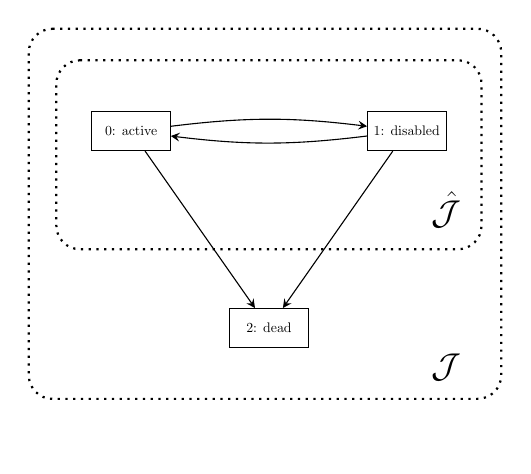
\begin{tikzpicture}[scale = 0.5, transform shape]
			\begin{scope}[every node/.style={ minimum width = 2cm, minimum height = 1cm}]
				\node (0) [rectangle, draw] at (0, 0) {$\text{0: active}$};
				\node (1) [rectangle, draw] at (7, 0) {$\text{1: disabled}$};
				\node (2) [rectangle, draw] at (3.5, -5) {$\text{2: dead}$};
				;
				
			\end{scope}
			
			\begin{scope}[every node/.style={minimum width = 2cm, minimum height = 4cm}]
				\node (5) at (8, -2) {\fontsize{50}{60}\selectfont $\hat{\mathcal{J}}$};
			\end{scope}
			
			\begin{scope}[every node/.style={minimum width = 2cm, minimum height = 4cm}]
				\node (5f) at (8, -6) {\fontsize{50}{60}\selectfont $\mathcal{J}$};
			\end{scope}
			
			\begin{scope}[>={stealth[black]},
				every edge/.style = {draw = black}]
				\path [->] 	(0) edge [bend left = 7] node {} (1)
				(0) edge [] node {} (2)
				(1) edge [] node {} (2)
				(1) edge [bend left = 7] node {} (0);
			\end{scope}
			
			
			
			
			\draw [rounded corners = 3mm, thick, dotted, scale=1]
			($(2) + (-5.4, 6.8)$) --
			($(2) + (5.4, 6.8)$) --
			($(2) + (5.4, 2)$) --
			($(2) + (-5.4, 2)$)
			--cycle;
			
			\draw [rounded corners = 3mm, thick, dotted, scale=1]
			($(2) + (-6.1, 7.6)$) --
			($(2) + (5.9, 7.6)$) --
			($(2) + (5.9, -1.8)$) --
			($(2) + (-6.1, -1.8)$)
			--cycle;
			
		\end{tikzpicture}
		\caption{Active-disabled-dead model.}
		\label{fig: 3stateEx}
	\end{center}
\end{figure}

Assume that there are no guaranteed payments, i.e. $B^\circ=0$. The policy holder saves for her retirement via the cash-dividend payment stream $D_1$ in the following manner

\begin{align*}
	dD_1(t) =& - \1{t<R} \1{Z(t)=0} \pi(t) \\
	&+ \1{t \geq R} \left( \1{Z(t)=0} + \1{Z(t)=1} \right) \frac{Y(t)}{a(t)}
\end{align*}

In words, the policy holder pays the total premium $\pi(t)$ directly into the surplus while active. As retired, a pension benefit rate is then paid out continuously as a fraction of the surplus $Y$. Since the surplus is forfeited upon death, we let $Y$ accrue not only with the rate of return $r$, but also with the mortality rate $\mu_{02}$ respectively $\mu_{12}$. This means that the surpluses of the deceased are inherited by the survivors.

Note that in this contract, no additional units of any payment stream $B^\dagger$ are purchased, so $D_2=Q=0$. Since we also have $B^\circ=0$, this means that $X=0$. In other words, we only have to project the 1-dimensional process $\tilde{Y}_j(t)$. Much more complex contracts could of course be envisioned following the blueprint of the preceding section. But the aim of this example is to lay bare the fundamental difference between fixed- and restricted path prognoses, and it is the view of this thesis that this is best done in a simple setting where every step can be intuitively interpreted.

The surplus has dynamics

\begin{align} \label{YExampleDyn}
\begin{split}
		dY(t) =& \left( r(t) + \mu_{Z(t)2}(t) \right) Y(t) dt \\
	&+ \1{t<R} \1{Z(t)=0} \pi(t) dt \\
	&- \1{t \geq R} \left( \1{Z(t)=0} + \1{Z(t)=1} \right) \frac{Y(t)}{a(t)} dt \\
	&- Y(t-) dN_2(t).
\end{split}
\end{align}

The quantity $a$ is the annuity

\begin{align*}
	a(t) = \int_t^n e^{-\int_t^s \bar{r}_t(u) + \bar{\mu}_t(u) du} ds
\end{align*}

where $\bar{r}_t(u)$ is the payout interest rate curve ("beregningsrenten") and $\bar{\mu}_t(u)$ is the payout mortality rate curve. These curves are updated regularly (e.g. yearly) and are examples of future management actions relevant in the context of prognoses. So in a stochastic model of the financial market, these curves will be adapted to the state market process.

\begin{remark}
	As we shall see, the choice of $\bar{r}_t(u)$ and $\bar{\mu}_t(u)$ has great impact on how the surplus is paid out over the course of retirement:

\begin{itemize}
	\item If $\bar{r}_t(u)<r(u)$ and $\bar{\mu}_t(u)<\mu_{02}(u),\mu_{12}(u)$ for $u \geq t$, the pension benefit rate $Y(t)/a(t)$ will tend to \textit{increase} over time.
	\item If $\bar{r}_t(u)>r(u)$ and $\bar{\mu}_t(u)>\mu_{02}(u),\mu_{12}(u)$ for $u \geq t$, the pension benefit rate $Y(t)/a(t)$ will tend to \textit{decrease} over time.
	\item If $\bar{r}_t(u)\approx r(u)$ and $\bar{\mu}_t(u)\approx \mu_{02}(u),\mu_{12}(u)$ for $u \geq t$, the pension benefit rate $Y(t)/a(t)$ will be approximately constant (see XXX for proof'ish).
\end{itemize}

Since $a(t) \underset{t \to n}{\longrightarrow} 0$, it follows that $a^{-1}(t) \underset{t \to n}{\longrightarrow} \infty$, which ensures that the surplus is eventually paid out.
\end{remark}

We are now ready to calculate prognoses. By equation (\ref{One}), the restricted path prognosis for the pension rate at some time $t \geq R$ is

\begin{align} \label{Naja}
\begin{split}
		\hat{b}^{\hat{\mathcal{J}}}(t) =& \econd[\frac{Y(t-)}{a(t)}]{Z(t-) \in \bar{\mathcal{J}}} \\
	=&\frac{\sum_{j \in \hat{\mathcal{J}}} \tilde{Y}_j(t)}{\sum_{j \in \hat{\mathcal{J}}} p_{0j}(0,t)} \frac{1}{a(t)} \\
	=&\frac{\tilde{Y}_0(t) + \tilde{Y}_1(t)}{p_{00}(0,t) + p_{01}(0,t)} \frac{1}{a(t)}.
\end{split}
\end{align}

Then by Proposition \ref{MainResult}, $\tilde{Y}_j(t) = \expec[\1{Z(t)=j} Y(t)]$ is described by the system of differential equations

\begin{align} \label{Jaja}
\begin{split}
	\frac{\partial}{\partial t} \tilde{Y}_0(t) =& \left( r(t) + \mu_{02}(t) - \1{t \geq R} \frac{1}{a(t)}\right) \tilde{Y}_0(t) \\
	&+ p_{00}(0,t) \1{t<R} \pi(t) \\
	&+ \mu_{10}(t) \tilde{Y}_1(t) - \mu_{01}(t) \tilde{Y}_0(t) - \mu_{02}(t) \tilde{Y}_0(t), \\
	\frac{\partial}{\partial t} \tilde{Y}_1(t) =& \left( r(t) + \mu_{12}(t) - \1{t \geq R} \frac{1}{a(t)}\right) \tilde{Y}_1(t) \\
	&+ \mu_{01}(t) \tilde{Y}_0(t) - \mu_{10}(t) \tilde{Y}_1(t) - \mu_{12}(t) \tilde{Y}_1(t).
\end{split}
\end{align}

Obviously, $\tilde{Y}_0(0)=\tilde{Y}_1(0)=0$ and $\tilde{Y}_2(t)=0$ (since the surplus is forfeited upon death). Note that the quantity $\mu_{02}(t) \tilde{Y}_0(t)$ appear with both a positive and a negative sign in the differential equation for $\tilde{Y}_0$ (and $\mu_{12}(t) \tilde{Y}_1(t)$ for $\tilde{Y}_1$). The positive contribution is from the surpluses inherited when other policy holders die. The negative contribution is from the infinitesimal probability of dying, thereby forfeiting her own surplus. These two effects cancel exactly.

We can also compute the fixed path prognosis for the path $z=0$, i.e. the prognosis obtained by assuming that the insured remains active and premium paying until retirement.  By Proposition \ref{FixedPath}, this prognosis is simply

\begin{align} \label{Naja2}
	\hat{b}^z(t) =& \frac{Y_z(t)}{a(t)}
\end{align}

where $Y_z(t)$ satisfies the differential equation

\begin{align} \label{Jaja2}
\begin{split}
		\frac{\partial}{\partial t}Y_z(t) =& \left( r(t) + \mu_{02}(t) - \1{t \geq R} \frac{1}{a(t)}\right) Y_z(t) \\
	&+ \1{t<R} \pi(t)
\end{split}
\end{align}

with $Y_z(0) = 0$. We now solve the restricted- and fixed path prognoses schemes schemes numerically for four different scenarios. The scenarios are:

\begin{itemize}
	\item \textbf{Baseline}: A best estimate scenario with premiums set at $\pi = 80$ t.DKK annually until retirement at $R=65$, a real return rate of 3\% per annum and transition intensities given as in (\ref{Intensities}). The payout interest rate $\bar{r}$ is constant at 3\% and the payout mortality rate $\bar{\mu}$ is equal to the realized active mortality, $\mu_{01}$.
	\item \textbf{Disability Stress}: The baseline scenario, \textit{but} with a higher disability intensity.
	\item \textbf{Longevity Stress}: The baseline scenario, \textit{but} with a lower mortality.
	\item \textbf{Interest Stress}: The baseline scenario, \textit{but} with a lower rate of return $r$ in the retirement phase.
\end{itemize}

Formally, the scenarios are:

\begin{table}[H]
	\caption{Four prognosis scenarios.}
	\begin{center}
	\begin{tabular}{ |c|c|c|c|c|c| }
		\hline
		Scenario & $\mu_{01}$ & $\mu_{10}$ & $\mu_{02}$ & $\mu_{12}$ & $r$ \\
		\hline
		Baseline & $\mu_{01}^{BE}(t)$ & $\mu_{10}^{BE}(t)$ & $\mu_{02}^{BE}(t)$ &$\mu_{12}^{BE}(t)$ & 0.03 \\
		Disability Stress & $1.5 \cdot \mu_{01}^{BE}(t)$ & $\mu_{10}^{BE}(t)$ & $\mu_{02}^{BE}(t)$ & $\mu_{12}^{BE}(t)$ & 0.03 \\
		Longevity Stress & $\mu_{01}^{BE}(t)$ & $\mu_{10}^{BE}(t)$ & $0.8 \cdot \mu_{02}^{BE}(t)$ & $0.8 \cdot \mu_{12}^{BE}(t)$ & 0.03 \\
		Interest Stress & $\mu_{01}^{BE}(t)$ & $\mu_{10}^{BE}(t)$ & $\mu_{02}^{BE}(t)$ & $\mu_{12}^{BE}(t)$ & $\1{t < R} 0.03 + \1{t \geq R} 0.02$ \\
		\hline
	\end{tabular}
\newline
\end{center}
\end{table}

\begin{figure}[H]
	\centering
	\caption{The development $\tilde{Y}_0$, $\tilde{Y}_1$ and $Y_z$ for the four scenarios, cf. equations (\ref{Jaja}) and (\ref{Jaja2}).}
	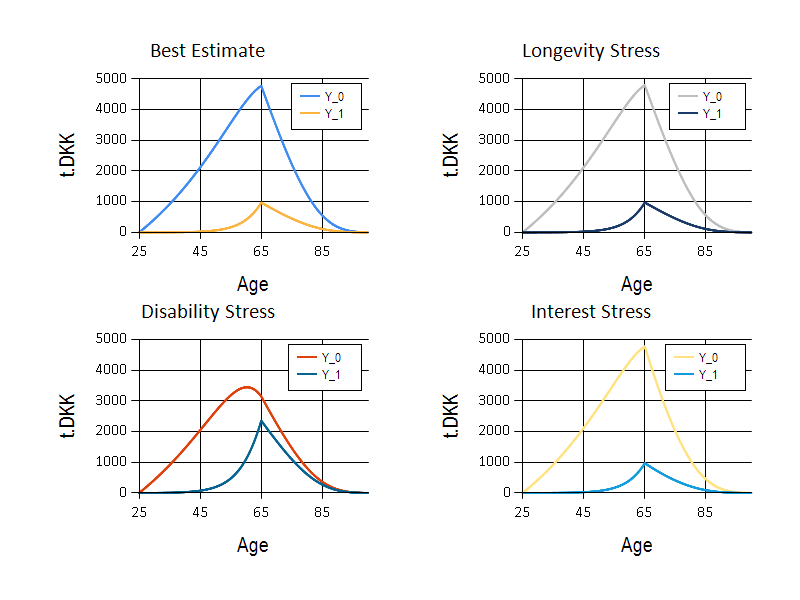
\includegraphics[width=\textwidth]{Reserves}
\end{figure}

\begin{itemize}
	\item For each scenario, the restricted path state-wise surpluses $\tilde{Y}_0$ and $\tilde{Y}_1$ are well below the fixed path surplus $Y_z$. This is because the state-wise surpluses $\tilde{Y}_j(t) = \expec[\1{Z(t)=j}Y(t)]$ include information on the transition probabilities via the indicator function. Recall that the $\tilde{Y}_j$'s are summed and normalized according to equation (\ref{Naja}) to obtain the restricted path prognoses.
	\item For the state-wise surpluses, the Disability Stress scenario differ the most from the other scenarios. This is because the policy holder is much more likely to enter the disabled, which increases $\tilde{Y}_1$ and decreases $\tilde{Y}_0$. Also, the disability intensity is so high for ages close to retirement that the intensity actually overpowers the return rate, which leads to a decreasing $\tilde{Y}_0$ \textit{before} retirement.
\end{itemize}

Next we graph the actual prognoses $\hat{b}^{\hat{\mathcal{J}}}$ and $\hat{b}^z$:

\begin{figure}[H] \label{FigureBens}
	\centering
	\caption{Annual benefit prognoses (fixed- and restricted path) for the four scenarios, cf. equations (\ref{Naja}) and (\ref{Naja2}).}
	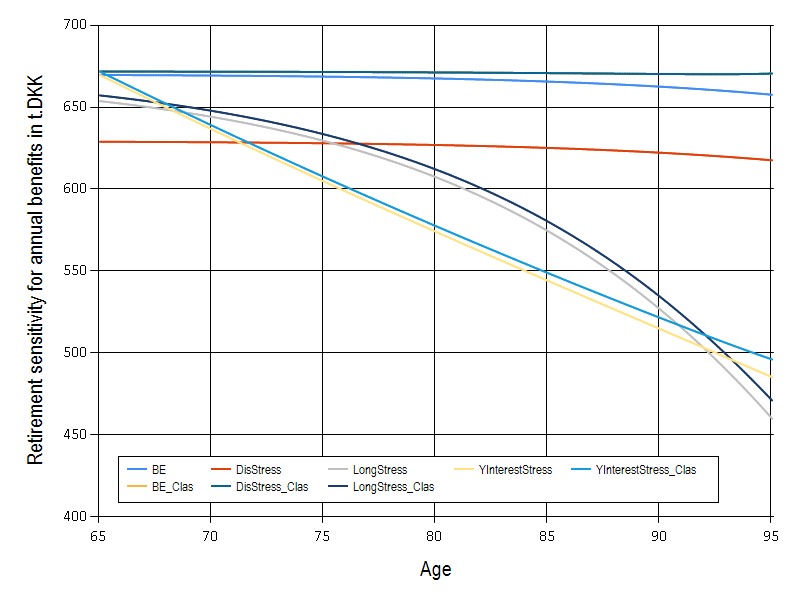
\includegraphics[width=\textwidth]{Benefits}
\end{figure}

A few things are worth noting in the Figure 5.3:

\begin{itemize}
	\item For each scenario, the classical prognosis is higher than the proposed prognosis $\hat{b}(t)$. This is what was expected and one of the principal reason for building the theory in the first place. The difference is, however, quite small -- and the inter-scenario variation is much larger.
	\item The difference between the BE- and the Disability Stress-scenario shows the promise of the proposed prognoses. When the disability rate is high, the insured is more likely to exit the premium paying state, which translates to a lower surplus at retirement. As noted earlier, an "unemployed"-state can be added to the state space, with an intensity that is probably much higher than the disability intensity.
	\item The Interest Stress scenario shows that if the payout interest rate $\bar{r}$ is set high than the realized rate, benefits decrease over time because the surplus is paid out "too quickly" in the early phase of retirement.
	\item The Longevity Stress scenario tells the same story, but with $\bar{\mu}$. Also, the start rate (at age 65) is lower in this scenario, because fewer people have died before retirement (their death would benefit the surpluses of the survivors). BEMÆRK KONKAVITET.
	\item Finally, note that BE\_Clas and DisStress\_Clas are exactly equal (and thus only one is visible on the graph) because only the technical disability rate $\mu_{01}^*$ is involved in the classical prognoses and this rate is not stressed.
\end{itemize}



\textbf{Remark om at lade premium afhænge af Y}

\textbf{Remark om at man nok skal have en unemployed state for at forskelle er store nok}

\subsubsection{Example Continued -- Premium Waiver} \label{Waiver}

In the last section, we saw how periods of disability can negatively impact the pension benefits paid out. It is in the interest of most policy holders to get rid of this risk. One way of achieving this is with a premium waiver ("indbetalingssikring"/"præmiefritagelse"). The idea is that the company assumes the premium payments in the disabled state, ensuring that savings increase at the same pace as in the active state.

Continuing the contract from the last section, we formalize the idea of a premium waiver as follows: The policy holder is still paying the premium rate $\pi(t)$ as active. From this is deducted the payment $q(t)$, which covers the premium waiver. The residual $\pi(t) - q(t)$ is then paid into the surplus $Y$.

The premium waiver must ensure that the same quantity, $\pi(t) - q(t)$, is paid into $Y$ as disabled. The $q(t)$ can then be determined under technical equivalence as a solution to 

\begin{align*}
	\int_0^R e^{-\int_0^s r^*(u)du}  p_{01}^*(0,s) \left( \pi(s) - q(s) \right) ds = \int_0^R e^{-\int_0^s r^*(u)du} p^*_{00}(0,s) q(s) ds,
\end{align*}

which just states that the expected present value of the premium waiver cover -- the left hand side -- must be equal to the expected present value of the \textit{payment} for the cover -- the right hand side.

\begin{remark}
	In the simple case where all payment functions are constant, we can isolate $q$ as

\begin{align*}
	q = \pi \frac{\int_0^R e^{-\int_0^s r^*(u)du} p_{01}^*(0,s) ds}{\int_0^R e^{-\int_0^s r^*(u)du} \left(p_{00}^*(0,s) + p_{01}^*(0,s)\right) ds}.
\end{align*}

Intuitively, this payment for the premium waiver cover is increasing in $p_{01}^*$ -- as it is then more likely that the cover will be activated -- and decreasing in $p_{00}^*$ -- as it is then less likely.
\end{remark}

As mentioned, the rate paid into the surplus $Y$ -- as active as well as disabled -- is then $\pi(t) - q(t)$. Consulting equation (\ref{YExampleDyn}), we see that $Y$ then has dynamics

\begin{align*}
\begin{split}
	dY(t) =& \left( r(t) + \mu_{Z(t)2}(t) \right) Y(t) dt \\
	&+ \1{t<R} \left( \1{Z(t)=0} + \1{Z(t)=1} \right) \left(\pi(t) - q(t) \right) dt \\
	&- \1{t \geq R} \left( \1{Z(t)=0} + \1{Z(t)=1} \right) \frac{Y(t)}{a(t)} dt \\
	&- Y(t-) dN_2(t).
\end{split}
\end{align*}

With the added assumptions that

\begin{itemize}
	\item $\mu_{02}(t) = \mu_{12}(t)$, meaning that the accrual from the surpluses of deceased happens at the same rate as active and as disabled,
\end{itemize}

then there is no distinction between the policy holder being in the active or the disabled state. The premium waiver effectively erases the risk from the transitions $0 \to 1$ (disability) and $1 \to 0$ (reactivation) from the point of view of the policy holder. No matter her state path inside $\hat{\mathcal{J}} = \{ 0,1 \}$, her surplus will develop at the same rate.

The computation of the prognosis can now be simplified by noting that

\begin{align*}
	\frac{\partial}{\partial t} \left(\tilde{Y}_0(t) + \tilde{Y}_1(t)\right) =& \left( r(t) + \mu_{02}(t) - \1{t \geq R} \frac{1}{a(t)}\right) \left(\tilde{Y}_0(t) + \tilde{Y}_1(t)\right) \\
	&+ \left(p_{00}(t) + p_{01}(t)\right)\1{t<R}\left(\pi(t) - q(t)\right) \\
	&- \mu_{02}(t) \left(\tilde{Y}_0(t) + \tilde{Y}_1(t)\right) \\
	=& \left( r(t) - \1{t \geq R} \frac{1}{a(t)}\right) \left(\tilde{Y}_0(t) + \tilde{Y}_1(t)\right) \\
	&+ \left(p_{00}(t) + p_{01}(t)\right)\1{t<R}\left(\pi(t) - q(t)\right),
\end{align*}

which is obtained by adapting (\ref{Jaja}) to the case with premium waiver. Solving this, the restricted path prognosis can be readily calculated as

\begin{align*}
	\hat{b}^{\hat{\mathcal{J}}}(t) =& \econd[\frac{Y(t-)}{a(t)}]{Z(t-) \in \bar{\mathcal{J}}} \\
	=&\frac{\sum_{j \in \hat{\mathcal{J}}} \tilde{Y}_j(t)}{\sum_{j \in \hat{\mathcal{J}}} p_{0j}(0,t)} \frac{1}{a(t)} \\
	=&\frac{\tilde{Y}_0(t) + \tilde{Y}_1(t)}{p_{00}(t) + p_{01}(t)} \frac{1}{a(t)}.
\end{align*}

The simplification is that we no longer have to solve a system of differential equations -- only the single one for $\tilde{Y}_0(t) + \tilde{Y}_1(t)$.

\begin{remark}
	In the construction of the premium waiver cover, we have assumed that it is priced under technical equivalence and that there is no contribution to the surplus as the return rate and the intensities $(r,\mu)$ are realized more favourably than assumed in the technical basis $(r^*,\mu^*)$. The assumption is made to make the mathematics more tractable and easier to interpret intuitively. In a more detailed contract, a favourable realization of $(r,\mu)$ would be paid back to the policy holder via the contribution process $C$ as described in Section \ref{WithProfit}. However, if $(r,\mu)=(r^*,\mu^*)$, then $C=0$ and so the results of Section \ref{Waiver} are exact.
\end{remark}

MÅSKE GRAF?

\subsection{Nominal Benefits Revisited}

We close the chapter on reserve-dependent benefits by showing that the prognoses for nominal benefits presented in Chapter \ref{ChapGuaranteedBen} can actually be replicated in the present reserve-dependent framework. Recall that the prospective technical reserve $V_{Z(t)}^*(t)$ for some payment stream $B$ has dynamics

\begin{align*}
	dV_{Z(t)}^*(t) =& r^*(t) V_{Z(t)}^* dt - b_{Z(t-)}(t) dt - \sum_{k \in \mathcal{J} \atop k \neq Z(t-)} R_{Z(t-)k}^*(t) \mu_{Z(t-)k}^*(t) dt \\
	&+ \sum_{k \in \mathcal{J} \atop k \neq Z(t-)} \left( V_k^*(t) - V_{Z(t-)}^*(t) \right) dN_k(t) - \triangle B_{Z(t-)}(R) d\varepsilon_{R}(t).
\end{align*}

which is clearly on the form (\ref{WDynamicsStart}). Assuming that $B$ satisfies the equivalence principle under the technical basis $(r^*,\mu^*)$, the initial value is $V_{Z(0)}^*(0)=0$. Then, by Proposition \ref{MainResult},

\begin{align*}
	\tilde{V}_j^*(t) = \expec[\1{Z(t)=j} V_{Z(t)}^*(t)] = p_{0j}(0,t) V_j^*(t)
\end{align*}

is characterized by the system of differential equations STJERNER PÅ P'er

\begin{align*}
	\frac{\partial}{\partial t} \tilde{V}_j^*(t) =& XXX\left( r^*(t) + \sum_{k \in \mathcal{J} \atop k \neq j} \mu_{jk}^*(t) \right) \tilde{V}_j^*(t) - p_{0j}(0,t) \left( b_j(t) + \sum_{k \in \mathcal{J} \atop k \neq j} \mu_{jk}^*(t) \left( b_{jk}(t) + V_k^*(t) \right) \right) \\
	&+ \sum_{k \in \mathcal{J} \atop k \neq j} \mu_{kj}(t) \left( \tilde{V}_k^*(t) + p_{0k}(0,t) V_k^*(t) \right) \\
	&+ \sum_{k \in \mathcal{J} \atop k \neq j} \left( \mu_{kj}(t) \tilde{V}_k^*(t) - \mu_{jk}(t) \tilde{V}_j^*(t) \right)XXX \\
	=& r^*(t) \tilde{V}_j^*(t) - p_{0j}(0,t) b_j(t) - \sum_{k \in \mathcal{J} \atop k \neq j} p_{0k}(0,t) \mu_{kj} b_{kj}(t) \\
	&+ \sum_{k \in \mathcal{J} \atop k \neq j} \left( \mu_{kj}(t) \tilde{V}_k^*(t) - \mu_{jk}(t) \tilde{V}_j^*(t) \right),
\end{align*}

with gluing condition

\begin{align*}
	\tilde{V}_j^*(R) =& \tilde{V}_j(R-) - p_{0j}(0,R) \triangle B_j(R)
\end{align*}

and initial value

\begin{align*}
	\tilde{V}_j^*(0) =& \1{j=0} V_{Z(0)}^*(t) \\
	=& 0
\end{align*}

In \cite{Lollike}, the authors show that XXX

To obtain the prognoses of the last chapter, define the payment stream

\begin{align*}
	d\bar{B}(t) = \frac{1}{V_{Z(t)}^*(t)}dB(t),
\end{align*}

we can prognosticate the payment stream

\begin{align*}
	V_{Z(t)}^*(t) d\bar{B}(t),
\end{align*}

which is clearly on the form (\ref{TotalPaymentStream}). By (XXX), the sojourn benefit prognosis is then

\begin{align*}
	\hat{\bar{b}}(t) =& \frac{\sum_{j \in \hat{\mathcal{J}}} \tilde{V}_j^*(t) \bar{b}_j(t)}{\sum_{j \in \hat{\mathcal{J}}} p_{Z(t_0)j}(t_0,t)} \\
	=& \frac{\sum_{j \in \hat{\mathcal{J}}} p_{0j}(0,t) V_j^*(t) \frac{b_j(t)}{V_j^*(t)}}{\sum_{j \in \hat{\mathcal{J}}} p_{Z(t_0)j}(t_0,t)} \\
	=& \frac{\sum_{j \in \hat{\mathcal{J}}} p_{0j}(0,t) b_j(t)}{\sum_{j \in \hat{\mathcal{J}}} p_{Z(t_0)j}(t_0,t)},
\end{align*}

which we recognize as the sojourn prognosis for the guaranteed payments from the last chapter, cf. (XXX). So in effect, the case with reserve-dependent benefits is a generalization of the case with guaranteed benefits.

\begin{remark}
	Dynamikken må gerne afhænge af hele den fortidige Z-sti
\end{remark}



XXXXX
\begin{table}[]
	\begin{tabular}{lll}
	Tabel med prognoser for nominal/reservedep og fixed/restric	&  &  \\
		&  &  \\
		&  & 
	\end{tabular}
\end{table}

\newpage
\section{Sensitivities -- Reserve-Dependent Benefits}

In recent years, the question of retirement age has been vividly discussed in the Danish public. The main issue is whether workers of certain professions -- typically hard physical labor -- can (or rather, should) remain in the workforce until the rather high pension ages laid down in the 2006 political settlement Velfærdsforliget. For these groups, sensitivities are of great interest\footnote{Of course, the public discussion has focused on state pensions which are pay-as-you-go systems.}, as they reveal the trade-offs between premiums paid, time of retirement and benefits received.

Having defined the prognoses, we will now formalize the concept of prognosis sensitivities. The point is to give the policy holder an idea of how much she can expect her benefits to increase if she postpones her time of retirement or if she increases premiums paid. And -- conversely -- how much she can expect her benefits to \textit{decrease} if she retires at an \textit{earlier} point in time or if she \textit{decreases} premiums paid.

We focus on only two kinds of sensitivities in this thesis -- time of retirement and premium level. However, the techniques presented can be used to obtain sensitivities for many other contract elements.

The point of retirement is already formalized as $R$. We will now formalize what we mean by premium level. Given a payment stream $B$, we assume that the premium (i.e. negative) part of the payment stream takes the form

\begin{align*}
	dB^-(t, \alpha) = \alpha \cdot dB^-(t),
\end{align*}

where $\alpha>0$ is the premium level. The sensitivities are now simply defined as the derivatives of the prognoses in $R$ and $\alpha$, respectively. For the case with reserve-dependent benefits, these are

\begin{align*}
	\frac{\partial}{\partial \theta} \econd[W(t-)b_{Z(t-)}]{\{Z(s) \}_{0 \leq s < t} \in \bar{\mathcal{J}}}, \\
	\frac{\partial}{\partial \theta} \econd[W(R-) \triangle B_{Z(R-)}]{\{Z(s) \}_{0 \leq s < R} \in \bar{\mathcal{J}}}, \\
	\frac{\partial}{\partial \theta} \econd[W(t-)b_{Z(t-)k}]{\{Z(s) \}_{0 \leq s < t} \in \bar{\mathcal{J}}, Z(t) = k}.
\end{align*}

for  $\theta = R,\alpha$. Since we have already seen that the case with guaranteed benefits is a special case of the case with reserve-dependent benefits, we only treat the latter.

\newpage
\subsection{Fixed Path} \label{FixedSens}

For the entirety of Section \ref{FixedSens}, we assume that the policy holder remains active until retirement (and alive until age 100). In other words, we assume the fixed path $z=0$, where 0 is the active state.

Recall the Unit Link savings contract from Section \ref{Numerics} (without any premium waiver). Assuming that the policy holder remains active until retirement $R$, her savings can be described by the differential equation (recall equation (\ref{Jaja2}))

\begin{align} \label{ReserveDE}
	\begin{split}
		\frac{\partial}{\partial t}W(t) =& \left( r(t) + \mu(t) - \1{t \geq R} \frac{1}{a(t)}\right) W(t) \\
		&+ \1{t<R} \pi(t)
	\end{split}
\end{align}

where we have suppressed the subscripts on the mortality. The fixed path prognosis is (recall equation (\ref{Naja2}))

\begin{align*}
	\hat{b}(t) =& \frac{W(t)}{a(t)}
\end{align*}

where we have suppressed the $z$-subscripts. Again, the quantity $a$ is the annuity

\begin{align*}
	a(t) = \int_t^n e^{-\int_t^s \bar{r}_t(u) + \bar{\mu}_t(u) du} ds
\end{align*}

where $\bar{r}_t(u)$ is the payout interest rate curve ("beregningsrenten") and $\bar{\mu}_t(u)$ is the payout mortality rate curve.

\subsubsection{Retirement sensitivity}

Denote by $W(t,R)$ the savings at time $t$ given retirement at time $R$. With regard to the retirement sensitivity, i.e. infinitesimally postponing retirement, there are two interesting, but distinct sensitivities to consider:

\begin{itemize}
	\item The sensitivity of the pension benefit \textit{start} rate, i.e.
	
	\begin{align} \label{StartPens}
		\frac{\partial}{\partial R} \hat{b}(R) = \frac{\partial}{\partial R} \frac{W(R-,R)}{a(R)}.
	\end{align}

	\item The effect on the pension benefit rate at some fixed time point $t$ \textit{after} retirement, i.e.
	
	\begin{align} \label{LaterPens}
		\frac{\partial}{\partial R} \hat{b}(t) = \frac{\partial}{\partial R} \frac{W(t-,R)}{a(t)}, \, \, t > R.
	\end{align}
	
\end{itemize}

The distinction is that in the first case, both the time of retirement and the time of payment are being moved infinitesimally. In the second case, only the time of retirement is moved whereas the time of payment is fixed.

\textbf{For the first case (\ref{StartPens})}, we can solve the differential equation (\ref{ReserveDE}) to obtain

\begin{align} \label{ReserveAtRetirement}
	W(R-,R) = \int_0^R e^{\int_s^R r(u) + \mu(u) du} \pi(s) ds
\end{align}

Differentiating, we obtain by Leibniz' integral rule

\begin{align*}
	\frac{\partial}{\partial R} W(R-,R) =& e^{\int_R^R r(u) + \mu(u) du} \pi(R) + \int_0^R \frac{\partial}{\partial R} e^{\int_s^R r(u) + \mu(u) du} \pi(s) ds \\
	=& \pi(R) + \left(r(R) + \mu(R)\right) W(R-,R)
\end{align*}

which has the intuitive interpretation that postponing retirement has the effect of increasing the saving \textit{at} retirement by the premium rate $\pi(R)$ and the rate of interest accrual $\left(r(R) + \mu(R)\right) W(R-,R)$. We also need the derivative of the annuity $a$, which  -- assuming the necessary differentiability -- is

\begin{align*}
	\frac{\partial}{\partial R} a(R) =& \frac{\partial}{\partial R} \int_R^n e^{-\int_R^s \bar{r}_R(u) + \bar{\mu}_R(u) du} ds \\
	=& - 1 + \int_R^n \frac{\partial}{\partial R} e^{-\int_R^s \bar{r}_R(u) + \bar{\mu}_R(u) du} ds \\
	=& - 1 + \int_R^n \left( \frac{\partial}{\partial R} \int_s^R \bar{r}_R(u) + \bar{\mu}_R(u) \right) e^{-\int_R^s \bar{r}_R(u) + \bar{\mu}_R(u) du} ds \\
	=& - 1 + \int_R^n \left( \bar{r}_R(R) + \bar{\mu}_R(R) + \int_s^R 	\frac{\partial}{\partial R} \left(\bar{r}_R(u)+\bar{\mu}_R(u)\right) du \right) e^{-\int_R^s \bar{r}_R(u) + \bar{\mu}_R(u) du} ds.
\end{align*}

The term

\begin{align*}
	\frac{\partial}{\partial R} \left(\bar{r}_R(u)+\bar{\mu}_R(u)\right)
\end{align*}

describes how the payout rates curves $\bar{r}_R(u)$ and $\bar{\mu}_R(u)$ change as more information is gained by postponing $R$. We will here assume that

\begin{itemize}
	\item $\frac{\partial}{\partial R} \bar{r}_R(u) = \frac{\partial}{\partial R} \bar{\mu}_R(u) = 0$ for $u > R$, i.e. that the information gained by postponing $R$ does not greatly change the curves $\bar{r}_R(u)$ and $\bar{\mu}_R(u)$. This assumption is certainly eligible for criticism and is an interesting research question in its own right. It is however outside the scope of this thesis.
\end{itemize}

Having made the assumption, we have

\begin{align*}
	\frac{\partial}{\partial R} a(R) =& - 1 +  \left(\bar{r}_R(R)+\bar{\mu}_R(R)\right) a(R)
\end{align*}

Then, by the quotient rule, the prognosis sensitivity for the pension benefit start rate is

\begin{align*}
	\frac{\partial}{\partial R} \hat{b}(R) =& \frac{\partial}{\partial R} \frac{W(R-,R)}{a(R)} \\
	=& \frac{\left( \pi(R) + \left(r(R) + \mu(R)\right) W(R-,R) \right) a(R) - W(R-,R) \left( \left(\bar{r}_R(R) + \bar{\mu}_R(R)\right) a(R) - 1 \right)}{\left( a(R) \right)^2} \\
	=& \frac{\pi(R) a(R)  + W(R-,R) + \left( r(R) - \bar{r}_R(R) + \mu(R) - \bar{\mu}_R(R) \right) W(R-,R) a(R)}{\left( a(R) \right)^2} \\
	=& \frac{\pi(R)  + W(R-,R) a^{-1}(R) + \left( r(R) - \bar{r}_R(R) + \mu(R) - \bar{\mu}_R(R) \right) W(R-,R)}{ a(R) }
\end{align*}

which is interpreted as follows: The numerator is the increment additional premium paid in $\pi(R)$ plus the increment benefit $W(R,R) a^{-1}(R)$ \textit{not} paid out, i.e. saved (hence the positive sign) plus the difference between the realized interest $r(R)$ and the payout interest $\bar{r}_R(R)$ weighted with the savings $W(R,R)$. So the sensitivity is the ratio between the infinitesimally additional savings and the annuity $a(R)$.

With the added assumption that

\begin{itemize}
	\item $\bar{r}_R (R) \approx r (R)$, i.e. that the payout interest rate curve initial value at retirement is close to the interest rate at retirement,
\end{itemize}

we then obtain

\begin{align*}
	\frac{\partial}{\partial R} \hat{b}(R) \approx \frac{\pi(R) + W(R-,R) a^{-1}(R)}{a(R)},
\end{align*}

which -- again -- is interpreted as the ratio between 1) the increment additional premium paid in $\pi(R)$ plus the increment benefit $W(R-,R) a^{-1}(R)$ saved, and 2) the annuity $a(R)$.

\textbf{For the second case (\ref{LaterPens})}, we can solve the differential equation (\ref{ReserveDE}) for $t>R$ as

\begin{align} \label{ReserveAfterRetirement}
	W(t-,R) =& W(R-,R) e^{\int_R^t r(u) + \mu(u) - a^{-1}(u) du},
\end{align}

which just says that the account at time $t>R$ is the account at retirement, positively compounded with interest and negatively compounded with benefits paid out. Differentiating, we obtain

\begin{align*}
	\frac{\partial}{\partial R} W(t-,R) =& \left( \pi(R) + \left(r(R) + \mu(R)\right) W(R-,R) \right) e^{\int_R^t r(u) + \mu(u) - a^{-1}(u) du} \\
	&+ W(R-,R) \left( - r(R) - \mu(R) + a^{-1}(R) \right) e^{\int_R^t r(u) + \mu(u) - a^{-1}(u) du} \\
	=& e^{\int_R^t r(u) + \mu(u) - a^{-1}(u) du} \left( \pi (R) + W(R-,R) a^{-1}(R) \right)
\end{align*}

which is interpreted as follows: By postponing retirement, an additional increment of $\pi(R)$ is paid in. Also, an increment \textit{less} of the benefit rate $W(R-,R) a^{-1}(R)$ is paid out, i.e. saved (hence the positive sign). These additional savings are then compounded (positively with $r$ and $\mu$ and negatively with $a^{-1}$) until time $t>R$.

The sensitivity of the pension benefit rate paid out at time $t>R$ is then

\begin{align*}
	\frac{\partial}{\partial R} \hat{b}(t) =& \frac{\partial}{\partial R} \frac{W(t-,R)}{a(t)} \\ =& \frac{e^{\int_R^t r(u) - a^{-1}(u) du} \left( \pi (R) + W(R-,R) a^{-1}(R) \right)}{a(t)}
\end{align*}

Note that this is consistent with the 

\begin{example}
As in Example \ref{Numerics}, premiums are set to 80 t.DKK (real) per annum starting at age 25. We consider three scenarios with varying real return rates; Low (1\%), Mean (3\%) and High (5\%). The table below then shows the value of the reserve at retirement at age 65, i.e. $W(R,R)|_{R=65}$ along with the start benefit $\hat{b}(R)|_{R=65}$.

\begin{center}
	\begin{tabular}{ |c|c|c|c|c| }
		\hline
		Scenario & $r$ & $\bar{r}$ & $W(R-,R)$ in m.DKK & $\hat{b}(R)$ in t.DKK \\
		\hline
		Low & 0.02 & 0.03 & 6.059 & 529 \\
		Mean & 0.03 & 0.03 & 7.691 & 671 \\
		High & 0.04 & 0.03 & 9.876 & 862 \\
		\hline
	\end{tabular}
\end{center}

Note that the payout interest rate $\bar{r}$ is the same in all three scenarios. This means that the scenarios differ not only on the realized interest rates $r$, but also on whether the payout interest rate $\bar{r}$ is fixed above or below the realized interest rate $r$. The result is the following figure:

\begin{figure}[H] \label{RSensiGraph}
	\centering
	\caption{Retirement sensitivity for the simple savings contract.}
	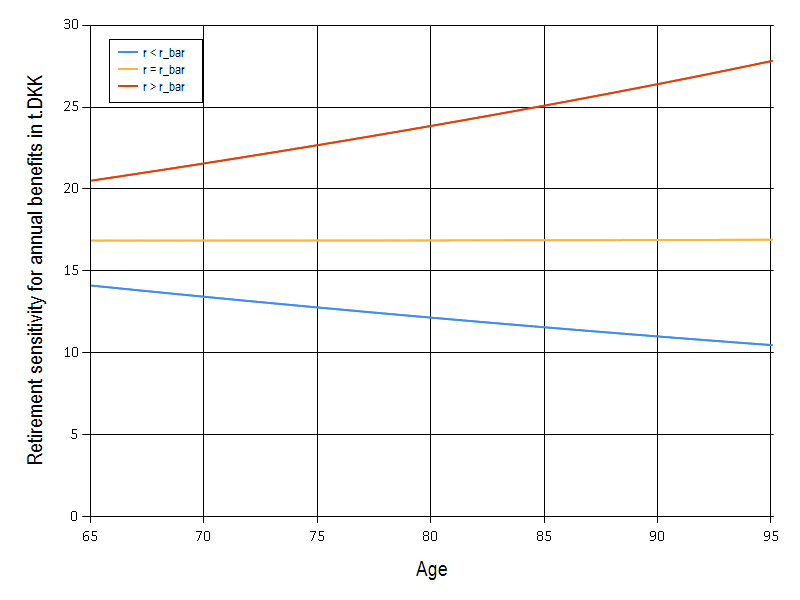
\includegraphics[width=\textwidth]{Rsensi}		
\end{figure}

There are at least two features worth noting on Figure \ref{RSensiGraph}:

\begin{itemize}
	\item As can be seen from the starting points of the three curves, the effect on the annual start benefit rate $\hat{b}(R)$ of postponing retirement one year is around 50-80 t.DKK on the annual rate (or equivalently 4-6 t.DKK effect on the monthly rate) -- depending on the rate of return in the savings phase. This figure is of interest to a policy holder considering whether to postpone retirement by a year.
	\item This postponement effect then increases/decreases/remains constant for later benefit rates $\hat{b}(t)$, $t>R$ depending on the scenario. For instance -- when $r < \bar{r}$ -- the retirement sensitivity decreases in time because the benefit rate does (as we saw in Example \ref{Numerics}). Intuitively, when most of the reserve is paid out in the early phase of retirement, increasing the reserve by postponing retirement matters most for these early benefit rates.
\end{itemize}
\end{example}

\subsubsection{Premium sensitivity}

Intuitively -- for the simple contract considered here -- if the policy holder, say, doubles her premiums, the prognosis should double as well. This makes sense because the only flow into or from the reserve until retirement is the premium stream. This is exactly what the following calculations show.

Assume that the premium rate takes the form

\begin{align*}
	\pi (t,\alpha) = \alpha \cdot \pi(t)
\end{align*}

where $\alpha$ is the premium level and $\pi(t)$ is some baseline premium plan. Denote by $W(t,R,\alpha)$ the reserve at time $t$ given retirement at time $R$ and a premium level of $\alpha$.

Consulting equations (\ref{ReserveAtRetirement}) and (\ref{ReserveAfterRetirement}), we see that

\begin{align*}
	W(t,R,\alpha) = \alpha W(t,R,1)
\end{align*}

and so

\begin{align} \label{AlphaDeriv}
	\frac{\partial}{\partial \alpha }W(t-,R,\alpha) = W(t-,R,1)
\end{align}

which just states that increasing the premium intensity increases the reserve at a rate constant in $\alpha$, which is equal to the reserve with the unscaled baseline premium plan. The sensitivity is then (for $t \geq R$)

\begin{align} \label{ResDeriv}
	\frac{\partial}{\partial \alpha }\frac{W(t-,R,\alpha)}{a(t)} = \frac{W(t-,R,1)}{a(t)},
\end{align}

which -- again -- is constant in $\alpha$.

\subsubsection{A contour map of benefits}

Having calculated the sensitivities (i.e. derivatives) of the prognosis benefit $\hat{b}(t,R,\alpha)$ in $R$ and $\alpha$, we have access to the gradient

\begin{align*}
	\nabla \hat{b}(t,R,\alpha) =
	\begin{bmatrix}
		\frac{\partial}{\partial \alpha }\hat{b}(t,R,\alpha) \\
		\frac{\partial}{\partial R }\hat{b}(t,R,\alpha)
	\end{bmatrix}
\end{align*}

for each $t \geq R$. With this, we can obtain a contour map of benefits, illustrating the trade-off between premium level $\alpha$ and time of retirement $R$. Premiums are again set at 80 t.DKK yearly beginning at age 25.

\begin{figure}[H] \label{ContourGraph}
	\centering
	\caption{A contour map of start benefits rates (i.e. the rate at retirement) as a function of premium level $\alpha$ and time of retirement $R$.}
	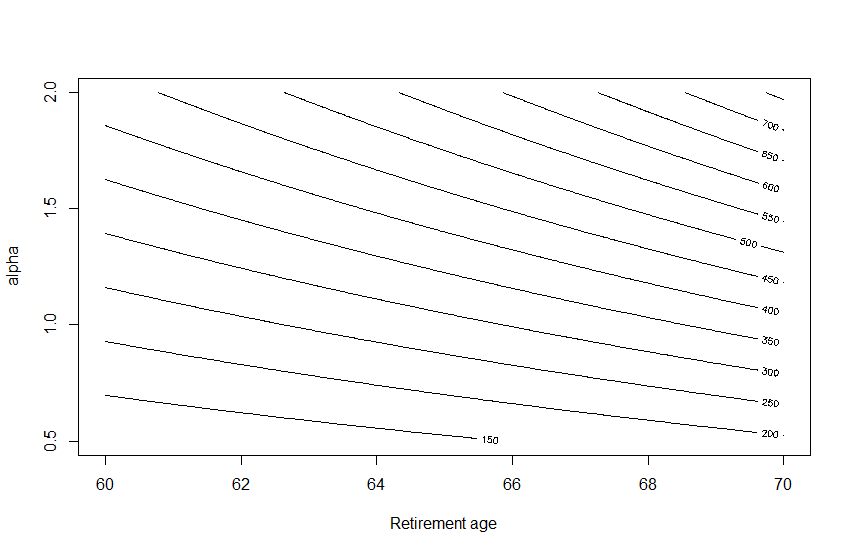
\includegraphics[width=\textwidth]{Contour}		
\end{figure}

Figure 6.2 shows the different avenues available (given that the pension scheme legislation is flexible enough) for obtaining a certain benefit level. This information is useful to the policy holder planning her retirement timing. Worth noting is:

\begin{itemize}
	\item The standard parameters $\alpha=1$ and $R=65$ gives a start benefit rate of around 670 t.DKK per annum, which is consistent with earlier results.
	\item From the bottom-left to the top-right the lines get increasingly close (going from one line to the next -- starting in the bottom left -- symbolizes an annual benefit rate increase of 200 t.DKK). This is because XXX.
\end{itemize}

\subsubsection{Exchange ratios}

Closely related to the contour map of the previous subsection, we consider the ratio between the sensitivities and denote it the \textit{exhange ratio}. The exchange ratio is of interest to the policy holder as it informs her how much -- infinitesimally -- she will have to increase her premiums in order to retire earlier \textit{while keeping the same benefit prognosis level}. This is a key piece of information for a policy holder deciding on her retirement timing.

\begin{definition}
	Given a benefit prognosis $\hat{b}(t,R,\alpha)$, the exchange ratio is defined as
	
\begin{align*}
	e(t,R,\alpha) = \frac{\frac{\partial}{\partial \alpha }\hat{b}(t,R,\alpha)}{\frac{\partial}{\partial R }\hat{b}(t,R,\alpha)}
\end{align*}
\end{definition}

In the simple contract pursued in this section, the exchange ratio for the prognosis at retirement is simply

\begin{align*}
	e(R,R,\alpha) =& \frac{\frac{\partial}{\partial \alpha }\frac{W(R-,R,\alpha)}{a(t)}}{\frac{\partial}{\partial R }\frac{W(R-,R,\alpha)}{a(t)}} \\
	=& \frac{\frac{W(R-,R,1)}{a(R)}}{\frac{\pi (R) + W(R-,R,\alpha) a^{-1}(R)}{a(R)}} \\
	=& \frac{W(R-,R,1)}{\pi (R) + W(R-,R,\alpha) a^{-1}(R)}
\end{align*}



\begin{remark}
	Midle før eller efter man tager brøken
\end{remark}

In the preceding section, intuitive results on sensitivities and exchange ratios were obtained for a simple savings contract. However, the setting had been without insurance event risk. The natural next step is to adapt the results of the preceding section to a setting with insurance risk.

\newpage
\subsection{Restricted Path}

When adding insurance risk, most quantities -- reserves, sensitivities, exchange ratios -- no longer have closed form solutions. Consequently, we have to settle for deriving systems of differential equations describing the sensitivities and solving them numerically.

Recall that the sojourn benefit rate prognosis is given by

\begin{align*}
	\hat{b}(t)=& \econd[\sum_{i=1}^n W_i(t-)b_{Z(t)}^i]{\{Z(s) \}_{0 \leq s < t} \in \bar{\mathcal{J}}} \\
	=& \frac{\sum_{j \in \hat{\mathcal{J}}} \tilde{W}_j(t-) b_j(t)}{\sum_{j \in \hat{\mathcal{J}}} p_{Z(t_0)j}(t_0,t)}.
\end{align*}

It it clear then that in order to calculate the sensitivities $\frac{\partial}{\partial \theta} \hat{b}(t,\theta)$ for $\theta=R,\alpha$, we need the sensitivities of the state-wise reserves, i.e.

\begin{align*}
	\frac{\partial}{\partial \theta} \tilde{W}_j(t,\theta) = \frac{\partial}{\partial \theta} \expec[\1{Z(t)=j} W(t)]
\end{align*}

Since we already have a system of differential equations describing $\tilde{W}_j(t,\theta)$, we can obtain an analogue system describing $\frac{\partial}{\partial \theta} \tilde{W}_j(t,\theta)$ by simply differentiating the differential equations, initial value and gluing condition of Proposition \ref{MainResult} with respect to $\theta$. The result is the following corollary:

\begin{corollary} \label{Corollary}
	For a process $W$ with initial value $w_0$ and dynamics
	
	\begin{align*}
		dW(t,\theta) =& f_{Z(t-)}(t,W(t-)) dt \\
		&+ \sum_{k \in \mathcal{J} \atop k \neq Z(t-)} g_{Z(t-)k}(t,W(t-)) dN_{k}(t) \\
		&+ h_{Z(t-)}(t,W(t-)) d \varepsilon_R(t),
	\end{align*}

	the $\theta$-sensitivity of the reserve
	
	\begin{align*}
		\frac{\partial}{\partial \theta} \tilde{W}_j(t) = \frac{\partial}{\partial \theta} \expec[\1{Z(t)=j} W(t)]
	\end{align*}
	
	is characterized by the system of differential equations NOT DONE
	
	\begin{align*}
		\frac{\partial}{\partial t} \frac{\partial}{\partial \alpha} \tilde{W}_j(t) =& f_j^1(t) \tilde{W}_j(t) + p_{0j}(0,t) f_j^0(t) \\
		&+ \sum_{k \in \mathcal{J} \atop k \neq j} \mu_{kj}(t) \left( g_{kj}^1(t) \tilde{W}_k(t) + p_{0k}(0,t) g_{kj}^0(t) \right) \\
		&+ \sum_{k \in \mathcal{J} \atop k \neq j} \left( \mu_{kj}(t) \tilde{W}_k(t) - \mu_{jk}(t) \tilde{W}_j(t) \right),
	\end{align*}
	
	for $t \in (0,R)\cup(R,n)$ and $j \in \mathcal{J}$. The initial values are
	
	\begin{align*}
		\tilde{W}_j(0) =& \1{j=0} w_0
	\end{align*}
	
	and the gluing conditions are
	
	\begin{align*}
		\tilde{W}_j(R) =& \tilde{W}_j(R-) + h_j^1(R) \tilde{W}_j(R-) + p_{0j}(0,R) h_j^0(R)
	\end{align*}
\end{corollary}

\begin{example}
	As a sanity check of the corollary, we can reproduce the results of the last section. So assume that $\mathcal{J} = \{ 0 \}$ and that
	
	\begin{align*}
		W(dt,R,\alpha) = r(t) W(t-,R,\alpha) + 1_{t<R} \alpha \cdot \pi(t) - 1_{t \geq R} W(t-,R,\alpha) b(t)
	\end{align*}

	Then by Corollary \ref{Corollary},
	
	\begin{align*}
		\frac{\partial}{\partial \alpha} \tilde{W}_0(t,R,\alpha) =&  \frac{\partial}{\partial \alpha} \expec[\1{Z(0)=j} W(t,R,\alpha)] \\
		=&\frac{\partial}{\partial \alpha} W(t,R,\alpha),
	\end{align*}

	is characterized by the differential equation
	
	\begin{align*}
		\frac{\partial}{\partial t} \frac{\partial}{\partial \alpha} W(t,R,\alpha) = \left\{
		\begin{array}{ll}
			r(t) \frac{\partial}{\partial \alpha} W(t,R,\alpha) + \pi(t) & \mbox{if } t < R \\
			\left( r(t) - b(t) \right) \frac{\partial}{\partial \alpha} W(t,R,\alpha) & \mbox{if } t > R
		\end{array}
		\right.,
	\end{align*}

	with gluing condition $\frac{\partial}{\partial \alpha} W(R,R,\alpha) = \frac{\partial}{\partial \alpha} W(R-,R,\alpha)$.
	
	Solving this differential equation, we obtain
	
	\begin{align*}
	\frac{\partial}{\partial \alpha} W(t,R,\alpha) =& \left\{
		\begin{array}{ll}
			\int_0^t e^{\int_s^t r(u) du} \pi(s) ds & \mbox{if } t \leq R \\
			\int_0^R e^{\int_s^R r(u) du} \pi(s) ds \cdot e^{\int_R^t r(u) - b(u) du} & \mbox{if } t > R
		\end{array}
		\right. \\
		=& W(t,R,1),
	\end{align*}

	where we used equation (\ref{WAlpha}). We see that this is exactly the sensitivity obtained in the last subsection (see equation (\ref{AlphaDeriv})). This check gives us confidence blah blah
	
	It may come as a surprise that $W(t,R,\alpha)$ does not depend on $\alpha$ at all. Note that this is \textit{only} the case because there are no benefits before retirement....
\end{example}


As noted earlier, one can replace $\alpha$ with another contract element to obtain other interesting sensitivities.

The derivative in $R$, however, poses a problem. Writing

\begin{align*}
	W(t) = W(t,R)
\end{align*}

to stress that the process depends on the fixed time of retirement $R$, we saw in chapter XXX that the function

\begin{align*}
	(t,R) \mapsto \tilde{W}(t,R) = \expec[\1{Z(t)}W(t,R)]
\end{align*}

is not differentiable on the line $t=R$, which means that the function

\begin{align*}
	(t,R) \mapsto \left. \frac{\partial}{\partial y} \tilde{W}(x,y) \right|_{(x,y)=(t,R)}
\end{align*}

is not well defined on the line $t=R$. However, the limits $\frac{\partial}{\partial R} \tilde{W}(t,R)$.

\begin{example}
	Consider a simple savings contract modelled on an alive-dead model. blah blah. By Proposition XX, we have
\end{example}

\begin{remark}
It is of course possible to decompose the premiums in the same manner as the benefits, i.e. into a scaled part (e.g. the premium rate) and a fixed part (e.g. the initial lump sum premium).
\end{remark}

\begin{remark}
How much $R$ decrease if premiums increase
\end{remark}

\begin{remark}
	remark om at man kunne bruge gennemsnitsløn istedet for at midle ud over Z
\end{remark}

\begin{example}
Continuation of Example \ref{ULExample} (Unit Link). Premium paid in is now $\alpha \cdot \pi(t)dt$

$\tilde{W}_j^\alpha(t)$ is characterized by

\begin{align*}
\frac{\partial}{\partial t} \tilde{W}_0^\alpha(t) =& \tilde{W}_0^\alpha(t) \left( R(t) - \1{t \geq R} b^\dagger(t) + \mu_{02}(t) \right) \\
&+ p_{00}(0,t) \1{t<R} \pi(t) \\
&+ \mu_{10}(t) \tilde{W}_1^\alpha(t) - \mu_{01}(t) \tilde{W}_0^\alpha(t) - \mu_{02}(t) \tilde{W}_0^\alpha(t), \, \, \tilde{W}_0^\alpha(0) = 0, \\
\frac{\partial}{\partial t} \tilde{W}_1^\alpha(t) =& \tilde{W}_1^\alpha(t) \left( R(t) - \1{t \geq R} b^\dagger(t) + \mu_{12}(t) \right) \\
&+ \mu_{01}(t) \tilde{W}_0^\alpha(t) - \mu_{10}(t) \tilde{W}_1^\alpha(t) - \mu_{12}(t) \tilde{W}_1^\alpha(t), \, \, \tilde{W}_1^\alpha(0) = 0,
\end{align*}

which is obtained by differentiating the system of differential equations for $\tilde{U}_j(t)$ with respect to $\alpha$. We obtain numerically the sensitivities

\begin{align*}
\frac{\partial}{\partial \alpha} \expec[W(t-) b_{Z(t)}(t) | Z(t) \in \hat{\mathcal{J}}] =& \frac{\sum_{j \in \hat{\mathcal{J}}} \frac{\partial}{\partial \alpha} \expec[W(t-) 1_{\{Z(t)=j\}}] b_j^{\dagger}(t)}{\sum_{j \in \hat{\mathcal{J}}} p_{0j}(0,t)} \\
=& \frac{\sum_{j \in \hat{\mathcal{J}}} \tilde{W}_j^\alpha(t) b_j^{\dagger}(t)}{\sum_{j \in \hat{\mathcal{J}}} p_{0j}(0,t)},
\end{align*}

\begin{figure}[H]
%	\includegraphics[width=\textwidth]{alphaDerivOLD}
	\caption{5 farver, 1 for hvert scenarie. Viser pensionsraters (årlige) afledte i $\alpha$, altså $\frac{\partial}{\partial \alpha} \expec[W(t-) b_{Z(t)}(t) | Z(t) \in \{0,1\}]$.Med andre ord stiger prognosen med ca 8.000 kr. årligt, hvis man øger sin indbetaling med 1\%. Årsagen til at prognosen ikke bare stiger lineært med $\alpha$ er naturligvis, at risikopræmierne til invalidedækningerne ikke afhænger af $\alpha$. Så når man betaler en krone marginalt går den direkte til livrenten. Så hvis hæver man sine præmier med 1\%, så hæver man prognosen med mere end 1\%.}
\end{figure}


\end{example}

\subsubsection{Exchange ratios}

In recent years, there has

Having calculated the prognosis sensitivities in time of retirement $R$ and premium level $\alpha$, an interesting derived quantity is the exchange ratio

\begin{align*}
	\frac{d \alpha (E)}{d R (E)}
\end{align*}

that is the rate by which the policy holder must increase her premium level in order to retire one year earlier with the same benefit rate. 

\newpage
\section{Suggestions for further research}

\begin{itemize}
	\item Higher moments
\end{itemize}

\newpage

\begin{appendices}

\section{Proof of Lemma \ref{Split}} \label{SplitProof}

Let $h>0$. Then

\begin{align} \label{NumDenom}
	\econd[\1{Z(t-h)=j} W(t-h)]{Z(t-h) \in \hat{\mathcal{J}}, Z(t) = k} = \frac{\expec[\1{Z(t-h)=j} \1{Z(t)=k} W(t-h)]}{\probability[Z(t-h) \in \hat{\mathcal{J}}, Z(t)=k]}
\end{align}

For the numerator in (\ref{NumDenom}), note that 

\begin{align*}
	\expec[\1{Z(t-h)=j} \1{Z(t)=k} W(t-h)] =& \mathbb{E} \left[ \econd[\1{Z(t-h)=j} \1{Z(t)=k} W(t-h)]{Z(t-h)} \right] \\
	=& \mathbb{E} \left[ \econd[\1{Z(t-h)=j} W(t-h)]{Z(t-h)} \econd[\1{Z(t)=k}]{Z(t-h)} \right] \\
	=& \sum_{i \in \mathcal{J}} p_{Z(t_0)i}(t_0,t-h) \econd[\1{Z(t-h)=j} W(t-h)]{Z(t-h)=i} \\
	&\times p_{ik}(t-h,t) \\
	=& \expec[\1{Z(t-h)=j} W(t-h)] p_{jk}(t-h,t)
\end{align*}

and for the denominator in (\ref{NumDenom}), note that 


\begin{align*}
	\probability[Z(t-h) \in \hat{\mathcal{J}}, Z(t)=k] = \sum_{i \in \mathcal{J}} p_{Z(t_0)i}(t_0,t-h) p_{ik}(t-h,t).
\end{align*}

Plugging these two results into (\ref{NumDenom}), we obtain

\begin{align*}
	\econd[\1{Z(t-h)=j} W(t-h)]{Z(t-h) \in \hat{\mathcal{J}}, Z(t) = k} =& \frac{\expec[\1{Z(t-h)=j} W(t-h)] p_{jk}(t-h,t)}{\sum_{i \in \mathcal{J}} p_{Z(t_0)i}(t_0,t-h) p_{ik}(t-h,t)} \\
	=& \frac{\expec[\1{Z(t-h)=j} W(t-h)] \frac{p_{jk}(t-h,t)}{h}}{\sum_{i \in \mathcal{J}} p_{Z(t_0)i}(t_0,t-h) \frac{p_{ik}(t-h,t)}{h}} \\
\end{align*}

Now letting $h$ tend to zero, we obtain the desired result by the following lemma:

\begin{lemma}
	\begin{align*}
		\lim_{h \searrow 0} \frac{p_{jk}(t-h,t)}{h} = \mu_{jk}(t).
	\end{align*}
\end{lemma}
\begin{proof}
	Since $x \mapsto p_{jk}(x,t)$ is continuous on $[0,t]$ and differentiable on $(0,t)$, there exists by the mean value theorem $\xi \in ( t-h, t)$ such that
	
	\begin{align*}
		\frac{-p_{jk}(t-h,t)}{h} =& \frac{p_{jk}(t,t)-p_{jk}(t-h,t)}{t-(t-h)} \\
		=& \frac{\partial}{\partial x} p_{jk}(x,t)|_{x=\xi} \\
		=& \mu_{j \bullet}(\xi) p_{jk}(\xi,t) - \sum_{i \in \mathcal{J} \atop i \neq j} \mu_{ji}(\xi) p_{ik}(\xi,t),
	\end{align*}
	
	where we also used Kolmogorov's backward differential equation. Now when $h \searrow 0$, we have $\xi \nearrow t$, and so
	
	\begin{align*}
		\lim_{h \searrow 0} \frac{p_{jk}(t-h,t)}{h} = \mu_{jk}(t),
	\end{align*}
	
	since $\mu_{jk}(t)$ is continuous (as $p_{jk}(x,t)$ is $C^{1,1}$).
\end{proof}

\newpage

\section{Proof of Proposition \ref{MainResult}} \label{MainProof}

Assume that $p_{Z(t_0)j}(t_0,t)>0$ for all $t>t_0$ and all $j \in \mathcal{J}$. We then have

\begin{align*}
    \tilde{W}_j(t) =& \expec[W(t) \1{Z(t)=j}] \\
    =& \expec[w_0 \1{Z(t)=j}] + \expec[\int_0^t \1{Z(t)=j} dW(s)] \\
    =& p_{Z(t_0)j}(t_0,t) \cdot w \\
    &+ \underbrace{\expec[\int_0^t \1{Z(t)=j} f_{Z(s-)}(s,W(s-)) ds]}_* \\
    &+ \underbrace{\expec[\int_0^t \sum_{k \in \mathcal{J} \atop k \neq Z(s-)} \1{Z(t)=j} g_{Z(s-)k}(s,W(s-)) dN_k(s)]}_{**} \\
    &+ \underbrace{\expec[\int_0^t \1{Z(t)=j} h_{Z(s-)}(s,W(s-)) d \varepsilon_{R}(s)]}_{***}.
\end{align*}

By Fubini's Theorem and the Tower Property, we then have

\begin{align*}
	* =& \int_0^t \mathbbm{E} \left[ \econd[\1{Z(t)=j} f_{Z(s-)}(s,W(s-))]{Z(s-)} \right] ds \\
	=& \int_0^t \sum_{i \in \mathcal{J}} p_{0i}(0,s-) \econd[\1{Z(t)=j} f_{i}(s,W(s-))]{Z(s-)=i} ds.
\end{align*}

For $**$ we have

\begin{align*}
	** =& \mathbbm{E} \left[ \econd[ \int_0^t \sum_{k \in \mathcal{J} \atop k \neq Z(s-)} \1{Z(t)=j} g_{Z(s-)k}(s,W(s-)) dN_k(s)]{Z(t)} \right] \\
	=& \expec[ \int_0^t \sum_{k \in \mathcal{J} \atop k \neq Z(s-)} \1{Z(t)=j} g_{Z(s-)k}(s,W(s-)) \1{Z(s-)=i} \mu_{ik}(s) \frac{p_{kj}(s,t)}{p_{ij}(s,t)} ds] \\
	=& \int_0^t \sum_{i \in \mathcal{J}} p_{0i}(0,s-) \sum_{k \in \mathcal{J} \atop k \neq i} \econd[\1{Z(t)=j} g_{ik}(s,W(s-))]{Z(s-)=i} \mu_{ik}(s) \frac{p_{kj}(s,t)}{p_{ij}(s,t)} ds,
\end{align*}

where we used that $g_{Z(s-)k}(s,W(s-))$ is predictable and that $\1{Z(-s) \neq k}\1{Z(t)=j}dN_k(s)$ has predictable compensator $\1{Z(t)=j} \sum_{i \in \mathcal{J} \atop i \neq k} \1{Z(s-)=i} \mu_{ik}(s) \frac{p_{kj}(s,t)}{p_{ij}(s,t)}$ (see \cite{Lollike}). EVT SKIFT I MED Z NOGET.

Finally, we have for $***$

\begin{align*}
	*** =& \mathbbm{E} \left[ \econd[\int_0^t \1{Z(t)=j} h_{Z(s-)}(s,W(s-)) d \varepsilon_{R}(s)]{Z(R-)} \right] \\
	=& \sum_{i \in \mathcal{J}} p_{0i}(0,R-) \econd[\int_0^t \1{Z(t)=j} h_{i}(s,W(s-)) d \varepsilon_{R}(s)]{Z(R-)=i} \\
	=& \1{t \geq R} \sum_{i \in \mathcal{J}} p_{0i}(0,R-) \econd[\1{Z(t)=j} h_{i}(R,W(R-))]{Z(R-)=i}
\end{align*}

Putting it all together, we have

\begin{align*}
    \tilde{W}_j(t) =& p_{Z(t_0)j}(t_0,t) \cdot w \\
    &+ \int_0^t \sum_{i \in \mathcal{J}} p_{0i}(0,s-) \econd[\1{Z(t)=j} f_{i}(s,W(s-))]{Z(s-)=i} ds \\
    &+ \int_0^t \sum_{i \in \mathcal{J}} p_{0i}(0,s-) \sum_{k \in \mathcal{J} \atop k \neq i} \econd[\1{Z(t)=j} g_{ik}(s,W(s-))]{Z(s-)=i} \mu_{ik}(s) \frac{p_{kj}(s,t)}{p_{ij}(s,t)} ds \\
    &+ \1{t \geq R} \sum_{i \in \mathcal{J}} p_{0i}(0,R-) \econd[\1{Z(t)=j} h_{i}(R,W(R-))]{Z(R-)=i} \\
\end{align*}

Now since $W(s-) \in  \mathcal{F}_{\left( 0,s- \right)}$ and $\1{Z(t)=j} \in \mathcal{F}_{\left( s-,\infty \right)}$, it follows by the Markovianity of $Z$ that

\begin{align*}
	W(s-) \indep \1{Z(t)=j} | Z(s-)
\end{align*}

and so

\begin{align*}
	\econd[\1{Z(t)=j}W(s-)]{Z(s-)=i} =& \econd[\1{Z(t)=j}]{Z(s-)=i} \econd[W(s-)]{Z(s-)=i} \\
	=& p_{ij}(s-,t) \frac{\tilde{W}_i(s-)}{p_{0i}(0,s-)}
\end{align*}


Using this and the affine structure of $f$, $g$ and $h$ we obtain

\begin{align}
\tilde{W}_j(t) =& p_{Z(t_0)j}(t_0,t) \cdot w \\
&+ \int_0^t \sum_{i \in \mathcal{J}} p_{0i}(0,s) p_{ij}(s,t) \left( f_i^0(s) + \frac{\tilde{W}_i(s-)}{p_{0i}(0,s)} f_i^1(s) \right) ds \\
&+ \int_0^t \sum_{i \in \mathcal{J}} p_{0i}(0,s) \sum_{k \in \mathcal{J} \atop k \neq i} \mu_{ik}(s) p_{kj}(s,t) \left( g_{ik}^0(s) + \frac{\tilde{W}_i(s-)}{p_{0i}(0,s)} g_{ik}^1(s) \right) ds \\
&+ \1{t \geq R}\sum_{i \in \mathcal{J}} p_{0i}(0,R) p_{ij}(R,t) \left( h_i^0(R) + \frac{\tilde{W}_i(R-)}{p_{0i}(0,R)} h_i^1(R) \right) \\
=& p_{Z(t_0)j}(t_0,t) \cdot w \label{FirstLineA} \\
&+ \int_0^t \sum_{i \in \mathcal{J}} p_{0i}(0,s) p_{ij}(s,t) f_i^0(s) ds \\
&+ \int_0^t \sum_{i \in \mathcal{J}} p_{ij}(s,t) \tilde{W}_i(s-) f_i^1(s) ds \\
&+ \int_0^t \sum_{i \in \mathcal{J}} p_{0i}(0,s) \sum_{k \in \mathcal{J} \atop k \neq i} \mu_{ik}(s) p_{kj}(s,t) g_{ik}^0(s) ds \\
&+ \int_0^t \sum_{i \in \mathcal{J}} \sum_{k \in \mathcal{J} \atop k \neq i} \mu_{ik}(s) p_{kj}(s,t) \tilde{W}_i(s-) g_{ik}^1(s) ds \\
&+ \1{t \geq R}\sum_{i \in \mathcal{J}} p_{0i}(0,R) p_{ij}(R,t) h_i^0(R) \label{FirstGlue} \\
&+ \1{t \geq R}\sum_{i \in \mathcal{J}} p_{ij}(R,t) \tilde{W}_i(R-) h_i^1(R) \label{SecondGlue}
\end{align}

$\tilde{W}_j(t)$ is not differentiable at $R$ for two reasons. First, the lump sum added via the $h$ function potentially renders $\tilde{W}_j(t)$ discontinuous at this point (and hence not differentiable). Second, even if $h=0$, the point $R$ is potentially a point of discontinuity for $f$ and $g$, which renders the integrals above non-differentiable. On $(0,R)\cup(R,n)$, however, we have by Leibniz' integral rule

\begin{align*}
\frac{\partial}{\partial t} \tilde{W}_j(t) =& \frac{\partial}{\partial t} p_{Z(t_0)j}(t_0,t) w_0 \\
&+ p_{Z(t_0j)}(t_0,t) f_j^0(t) \\
&+ \tilde{W}_i(t-) f_j^1(t) \\
&+ \sum_{i \in \mathcal{J} \atop i \neq j} p_{Z(t_0)i}(t_0,t) \mu_{ij}(t) g_{ij}^0(t) \\
&+ \sum_{i \in \mathcal{J} \atop i \neq j} \tilde{W}_i(t) \mu_{ij}(t) g_{ij}^1(t) \\
&+ \int_0^t \sum_{i \in \mathcal{J}} p_{0i}(0,s) \frac{\partial}{\partial t} p_{ij}(s,t) f_i^0(s) ds \\
&+ \int_0^t \sum_{i \in \mathcal{J}} \frac{\partial}{\partial t} p_{ij}(s,t) \tilde{W}_i(s-) f_i^1(s) ds \\
&+ \int_0^t \sum_{i \in \mathcal{J}} p_{0i}(0,s) \sum_{k \in \mathcal{J} \atop k \neq i} \mu_{ik}(s) \frac{\partial}{\partial t} p_{kj}(s,t) g_{ik}^0(s) ds \\
&+ \int_0^t \sum_{i \in \mathcal{J}} \sum_{k \in \mathcal{J} \atop k \neq i} \mu_{ik}(s) \frac{\partial}{\partial t} p_{kj}(s,t) \tilde{W}_i(s-) g_{ik}^1(s) ds \\
&+ \1{t \geq R}\sum_{i \in \mathcal{J}} p_{0i}(0,R) \frac{\partial}{\partial t} p_{ij}(R,t) h_i^0(R) \\
&+ \1{t \geq R}\sum_{i \in \mathcal{J}} \frac{\partial}{\partial t} p_{ij}(R,t) \tilde{W}_i(R-) h_i^1(R)
\end{align*}

We can now use the Kolmogorov forward equations

\begin{align*}
\frac{\partial}{\partial t} p_{Z(t_0)j}(t_0,t) = \sum_{i \in \mathcal{J} \atop i \neq j} \left( p_{Z(t_0)i}(t_0,t) \mu_{ij}(t) - \mu_{ji}(t) p_{Z(t_0)j}(t_0,t) \right)
\end{align*}

to recognize $\tilde{W}_j(s)$ and $\tilde{W}_i(s-)$ from equations (\ref{FirstLineA}) through (\ref{SecondGlue}) to arrive at

\begin{align*}
	\frac{\partial}{\partial t} \tilde{W}_j(t) =& p_{Z(t_0j)}(t_0,t) f_j^0(t) + \tilde{W}_i(t-) f_j^1(t) \\
	&+ \sum_{i \in \mathcal{J} \atop i \neq j} \mu_ij(t) \left( p_{Z(t_0)i}(t_0,t) g_{ij}^0(t) + \tilde{W}_i(t) g_{ij}^1(t) \right) \\
	&+ \sum_{i \in \mathcal{J} \atop i \neq j} \left( \tilde{W}_i(t) \mu_{ij}(t) - \mu_{ji}(t) \tilde{W}_j(t) \right)
\end{align*}

The initial value is just

\begin{align*}
	\tilde{W}_j(t_0) =& \expec[\1{Z(t_0=j)} W(0)] \\
	=& \1{j=Z(t_0)} \cdot w
\end{align*}

and by inspecting equations (\ref{FirstLineA}) through (\ref{SecondGlue}), the gluing condition at time $R$ follows from the continuity of the transition probabilities

\begin{align*}
	\tilde{W}_j(R) - \tilde{W}_j(R-) = p_{Z(t_0)j}(t_0,R) h_j^0(R) + \tilde{W}_j(R-) h_j^1(R)
\end{align*}

\end{appendices}

\newpage

\bibliographystyle{plain}
\bibliography{Speciale}

\end{document}